%-------------------------------------------------------
%-- PREAMBLE
%-------------------------------------------------------
\documentclass[8pt]{beamer}
\usetheme[]{Feather}
  
\setbeamersize{text margin left=0.75cm,text margin right=0.75cm}

% INCLUDE PACKAGES
%-------------------------------------------------------

\usepackage[utf8]{inputenc}
\usepackage[english]{babel}
\usepackage[T1]{fontenc}
\usepackage{helvet}

\usepackage{graphicx}
\graphicspath{ {imgs/} }

\usepackage[utf8]{inputenc}
\usepackage[english]{babel}
\usepackage[protrusion=true,expansion=true]{microtype} 
\usepackage{amsmath,amsfonts,amsthm,amssymb,bm}
\usepackage{color, xcolor}
\usepackage{listings}
\usepackage[document]{ragged2e}
\usepackage{wrapfig}
\usepackage[printwatermark]{xwatermark}
\usepackage{subcaption}
\usepackage{mdframed}
\usepackage{multicol}
\usepackage{environ}
\usepackage{tikz, pgfplots}
\usepackage{framed}

\lstset{
    backgroundcolor=\color[rgb]{0.86,0.88,0.93},
    language=matlab, keywordstyle=\color[rgb]{0,0,1},
    basicstyle=\footnotesize \ttfamily,breaklines=true,
    escapeinside={\%*}{*)}
}

% DEFFINING COLORS
%-------------------------------------------------------
\definecolor{glgRed}{RGB}{214,45,32}
\definecolor{glgGreen}{RGB}{0,135,68}
\definecolor{glgBlue}{RGB}{0,87,231}
\definecolor{glgOrange}{RGB}{255,167,0}

\definecolor{retroBrown}{RGB}{102,101,71}
\definecolor{retroRed}{RGB}{251,46,1}
\definecolor{retroGreen}{RGB}{111,203,159}
\definecolor{retroYellow}{RGB}{255,226,138}

\definecolor{pastelBlue}{RGB}{27,133,184}
\definecolor{pastelRed}{RGB}{174,90,65}
\definecolor{pastelGreen}{RGB}{85,158,131}
\definecolor{pastelBlack}{RGB}{90,82,85}

\definecolor{niceBlack}{RGB}{14,17,17}
\definecolor{niceBlue}{RGB}{14,104,206}

% Beamer Color Scheme
\setbeamercolor{Feather}{fg=niceBlack!20,bg=niceBlack!90}
\setbeamercolor{structure}{fg=niceBlack}
\setbeamercolor{frametitle}{bg=niceBlack!70}
\setbeamercolor{normal text}{fg=black!85}


% Tikz Macros
% --------------------------------------------------------------------
\usetikzlibrary{shapes,arrows, backgrounds, positioning, fit, decorations.pathmorphing}

\tikzstyle{sectionBlock} = [draw, fill=blue!20, rectangle, minimum height=3em, minimum width=3em]
\tikzstyle{block} = [draw, fill=white, rectangle, minimum height=3em, minimum width=3em]
\tikzstyle{sum} = [draw, fill=white, circle, node distance=1cm]
\tikzstyle{input} = [coordinate]
\tikzstyle{output} = [coordinate]
\tikzstyle{pinstyle} = [pin edge={to-,thin,black}]
\tikzstyle{mcCircle} = [draw, circle, line width=0.5mm, minimum width=3em, minimum height=3em, fill=white]
\tikzstyle{mcInput} = [draw, rectangle, line width=0.5mm, minimum width=3em, minimum height=3em, fill=black!10]
\tikzstyle{mcCircleX} = [draw=myBlue!80, circle, line width=0.75mm, minimum width=3em, minimum height=3em, fill=white]
\tikzstyle{mcCircleY} = [draw=myBlue!80, circle, line width=0.75mm, minimum width=3em, minimum height=3em, fill=white]


% DEFFINING AND REDEFINING COMMANDS
%-------------------------------------------------------

% colored hyperlinks
\newcommand{\chref}[2]{
  \href{#1}{{\usebeamercolor[bg]{Feather}#2}}
}

\makeatletter
\let\beamer@writeslidentry@miniframeson=\beamer@writeslidentry
\def\beamer@writeslidentry@miniframesoff{%
  \expandafter\beamer@ifempty\expandafter{\beamer@framestartpage}{}% does not happen normally
  {%else
    % removed \addtocontents commands
    \clearpage\beamer@notesactions%
  }
}
\newcommand*{\miniframeson}{\let\beamer@writeslidentry=\beamer@writeslidentry@miniframeson}
\newcommand*{\miniframesoff}{\let\beamer@writeslidentry=\beamer@writeslidentry@miniframesoff}
\makeatother

\makeatletter
\patchcmd{\beamer@sectionintoc}
  {\vfill}
  {\vskip\itemsep}
  {}
  {}
\makeatother  

% tensor 2:
\newcommand{\tend}[1]{\hbox{\oalign{$\bm{#1}$\crcr\hidewidth$\scriptscriptstyle\bm{\sim}$\hidewidth}}}
\newcommand{\tenq}[1]{\hbox{\oalign{$\bm{#1}$\crcr\hidewidth$\scriptscriptstyle\bm{\sim}$\hidewidth}}}


% ENVIROMENTS
%-------------------------------------------------------

\AtBeginSection[]{
  \begin{frame}
  \vfill
    \centering
    \Huge \color{niceBlack!85} \insertsectionhead\par%
  \vfill
  \end{frame}
}

%\AtBeginSubsection[]{
%  \begin{frame}
%  \vfill
%    \centering
%    \Huge \color{glgBlue!60} \insertsubsectionhead\par%
%    \huge \color{niceBlack!85} \insertsectionhead\par%
%  \vfill
%  \end{frame}
%}

\newenvironment<>{varblock}[2][.9\textwidth]{%
  \setlength{\textwidth}{#1}
  \begin{actionenv}#3%
    \def\insertblocktitle{#2}%
    \par%
    \usebeamertemplate{block begin}}
  {\par%
    \usebeamertemplate{block end}%
  \end{actionenv}}

\NewEnviron{myequation}{%
    \begin{equation*}
    \scalebox{1.1}{$\BODY$}
    \end{equation*}
    }
    
% INFORMATION IN THE TITLE PAGE
%-------------------------------------------------------

\title[Optimal Control: An application to a non-isothermal continuous reactor]
{
      Optimal Control:\\An application to a non-isothermal continuous reactor
}

\subtitle[]
{
}

\author[Otacílio Bezerra Leite Neto]
{      
	Otacílio Bezerra Leite Neto\\
}

\institute[]
{
	TI0153 - Trabalho de Conclusão de Curso II\\
    Department of Teleinformatics Engineering\\
    Federal University of Ceará - UFC\\
  
  %there must be an empty line above this line - otherwise some unwanted space is added between the university and the country (I do not know why ;( )
}

\date{\today}

%-------------------------------------------------------
%-- THE BODY OF THE PRESENTATION
%-------------------------------------------------------

\begin{document}

%-------------------------------------------------------
% THE TITLEPAGE
%-------------------------------------------------------

{ \1
\begin{frame}[plain,noframenumbering] % the plain option removes the header from the title page, noframenumbering removes the numbering of this frame only
  \titlepage % call the title page information from above
\end{frame}}

%-------------------------------------------------------
% SUMMARY
%-------------------------------------------------------

\begin{frame}
	\begin{center} \Large \bfseries
		Summary
	\end{center}
    \begin{columns}[t]
        \begin{column}{0.5\textwidth}
            \tableofcontents[sections={1-3}]
        \end{column}
        \begin{column}{0.5\textwidth}
            \tableofcontents[sections={4-6}]
        \end{column}
    \end{columns}
\end{frame}


%-------------------------------------------------------
% SECTION - Introduction
%-------------------------------------------------------
\section{Introduction}
%-------------------------------------------------------
\subsection{Contextualization}
%-------------------------------------------------------
\begin{frame}[c]{Introduction}{Contextualization}

\vskip0.25cm

\begin{itemize}
	\item We are discussing the \textbf{automatic control} of \textbf{dynamical systems}; \vskip0.2cm
	
	\item We are discussing \textbf{chemical reactor network systems}, for processes described as:\vskip0.2cm
	
	\begin{figure} \centering
		\resizebox{0.6\textwidth}{!}{\begin{tikzpicture}[auto, node distance=3cm, >=latex']
	\node [input] (input1) {};
	\node [input, below of=input1, node distance=1.5em] (input2) {};
	\node [input, below of=input2, node distance=1.5em] (input3) {};
	\node [block, right of=input2, minimum width=8em, minimum height=5em] (system) {{\large \bfseries System}};
	\node [output, right of=system] (output2) {};
	\node [output, above of=output2, node distance=1.5em] (output1) {};		
	\node [output, below of=output2, node distance=1.5em] (output3) {};
	
	\node [below of=system, node distance=6em] {$\left\{ \begin{matrix} \mathcal{R}^{(1)}  & \overset{K_{11}(T)}{\longrightarrow} & \cdots & \overset{K_{1n}(T)}{\longrightarrow} &  \mathcal{P}^{(1)} & & \Delta H_1 \\ \vdots &  & \vdots &  & \vdots  & &  \\ \mathcal{R}^{(N)} &  \overset{K_{n1}(T)}{\longrightarrow} & \cdots & \overset{K_{nn}(T)}{\longrightarrow} & \mathcal{P}^{(N)}  & & \Delta H_n \\ \end{matrix} \right.$};				
	
	\draw[->, line width=0.5mm] (input1) node[pos=0.1]{Reactants} -- (input1-|system.west);
	\draw[->, line width=0.5mm] (input3) -- node[pos=0.1]{Heat Capacity} (input3-|system.west);
	\draw[<-, line width=0.5mm] (output1) -- node[pos=0.1,yshift=1.5em]{Products} (output1-|system.east);
	\draw[<-, line width=0.5mm] (output3) -- node[pos=0.1,yshift=1.5em]{Temperature} (output3-|system.east);
\end{tikzpicture}}
	\end{figure} \vskip0cm
	
	\item Optimal control theory has been revisited from several innovative fields in the last years {\bfseries \cite{Cairano:2014, Tang:2016, Eren:2017}}. Furthermore, reactor systems are subject of active research, with several open challenges {\bfseries \cite{Gupta:2012, Mulas:2015}}.
\end{itemize}

\end{frame}

%-------------------------------------------------------
\subsection{Problem Definition}
%-------------------------------------------------------
\begin{frame}[t]{Introduction}{Problem Definition}

\vskip0.25cm
\begin{itemize}
	\item The system used for the experiments was the non-isothermal Continuous Stirred Tank Reactor (CSTR) presented by {\bfseries \cite{Klatt:1998}}. \vskip0.25cm
\end{itemize}

\begin{center}
\begin{varblock}[1\textwidth]{Non-isothermal CSTR} \centering
	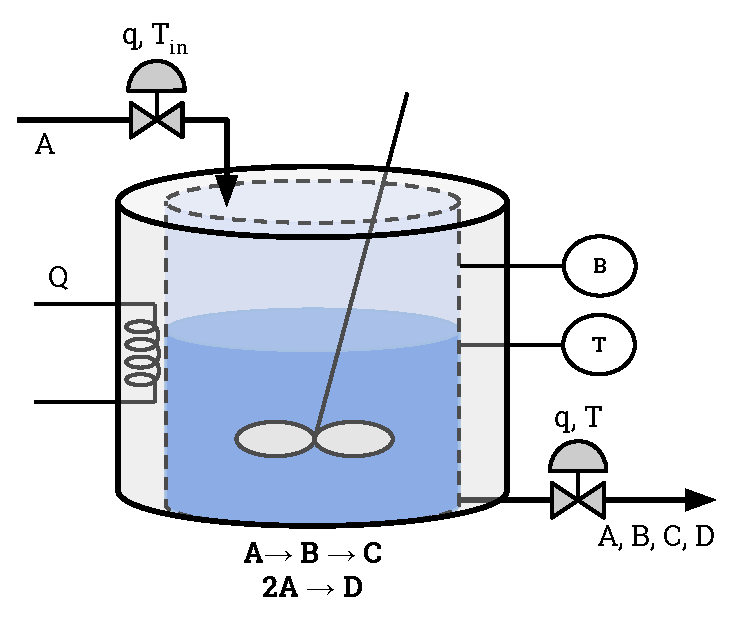
\includegraphics[width=0.5\textwidth]{exoCSTR}
\end{varblock}
\end{center} \vskip0.2cm

\end{frame}

%-------------------------------------------------------
\begin{frame}[t]{Introduction}{Problem Definition}

\vskip0.25cm
\begin{itemize}
	\item The system used for the experiments was the non-isothermal Continuous Stirred Tank Reactor (CSTR) presented by {\bfseries \cite{Klatt:1998}}. \vskip0.25cm
\end{itemize}	

\begin{center}
\begin{varblock}[1\textwidth]{Non-isothermal CSTR} \centering
	\begin{minipage}{.5\textwidth}
		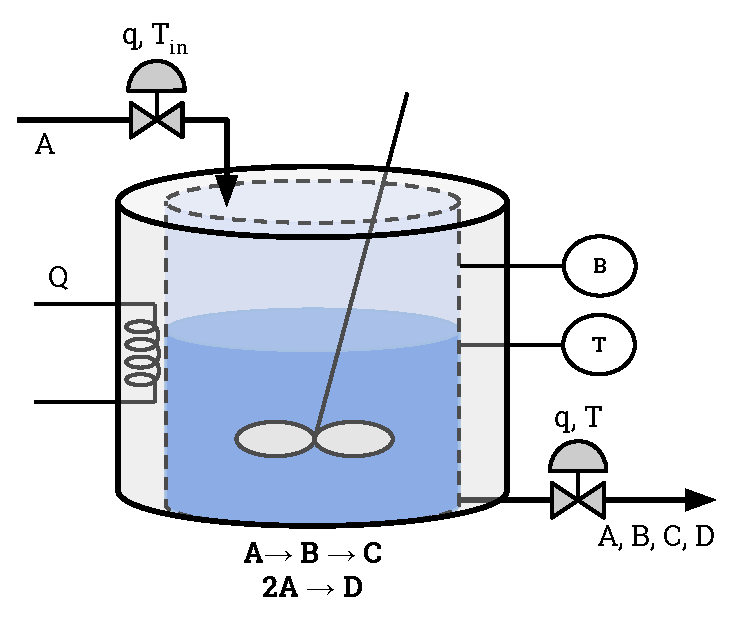
\includegraphics[width=\textwidth]{exoCSTR}
	\end{minipage}%
	\begin{minipage}{.5\textwidth}
		{\justifying \bfseries This system...} \vskip0.2cm
		
		\begin{itemize}
			\item characterizes a wide range of industrial applications;\vskip0.2cm
			
			\item is a classical benchmark for multiple-input multiple-output (MIMO) control systems;\vskip0.2cm
			
			\item is highly nonlinear, with non-minimum phase behavior and unmeasurable states;\vskip0.2cm
		\end{itemize}
	\end{minipage}
\end{varblock}
\end{center} \vskip0.2cm

\end{frame}

%-------------------------------------------------------
% SECTION - Dynamical System Analysis
%-------------------------------------------------------
\section{Dynamical System Analysis}
%-------------------------------------------------------
\subsection{Dynamical Models for Chemical Reactors}
%-------------------------------------------------------
\begin{frame}[t]{Dynamical System Analysis}{Mathematical Models for Chemical Reactors}

\vskip0.25cm

\begin{itemize}
	\item Dynamical systems are modelled through the Conservation Laws from physics;
\end{itemize}

\begin{varblock}[1\linewidth]{Mass Balance for Chemical Reactors}
	\begin{equation}
	\begin{split}
	    \begin{pmatrix}
	        \text{Accumulation} \\ \text{of mass} \\ \text{in the system}
	    \end{pmatrix} &=  \left[ \begin{pmatrix}
	        \text{Mass flow} \\ \text{entering} \\ \text{system}
	    \end{pmatrix} + \begin{pmatrix}
	        \text{Mass} \\  \text{produced} \\ \text{by reactions}
	    \end{pmatrix} \right] \\ &\ \ \ \ \ \  \ \ \ \ \ \ \ \ \ \ \ \ \ \ \ \ \ \ \  - \left[ \begin{pmatrix}
	        \text{Mass flow} \\ \text{leaving} \\ \text{system}
	    \end{pmatrix} + \begin{pmatrix}
	        \text{Mass} \\ \text{consumed} \\ \text{by reactions}
	    \end{pmatrix} \right]
	\end{split}
	\end{equation} \vskip0.2cm
\end{varblock}

\begin{varblock}[1\linewidth]{Conservation of Energy for Chemical Reactors}
	\begin{equation}
        \begin{pmatrix}
            \text{Accumulation} \\ \text{of thermal energy} \\ \text{in the system}
        \end{pmatrix} = \begin{pmatrix}
            \text{Heat flow} \\ \text{entering} \\ \text{the system}
        \end{pmatrix} - \begin{pmatrix}
            \text{Heat flow} \\ \text{leaving} \\ \text{the system}
        \end{pmatrix} + \begin{pmatrix}
            \text{Entropy} \\ \text{contribution} \\ \text{from reactions}
        \end{pmatrix}
    \end{equation} \vskip0.2cm
\end{varblock}

\end{frame}

%-------------------------------------------------------
\begin{frame}[t]{Dynamical System Analysis}{Mathematical Models for Chemical Reactors}

\vskip0.25cm

\begin{itemize}
	\item Assuming a continuous reactor of constant volume, comprised by a dilute solution of reactant and products...
\end{itemize}

\begin{varblock}[1\linewidth]{Mass Balance for Chemical Reactors}
	\begin{equation}
	\cfrac{d (\rho_A)}{dt} = q (\rho^{(A)}_{in} - \rho^{(A)}_{out}) + \left( \sum_{\alpha X \rightarrow \beta A} \cfrac{1}{\beta} K_{XA}(T) (\rho_X)^{\alpha} \right) - \left(\sum_{\alpha A \rightarrow \beta X} \cfrac{1}{\beta} K_{AX}(T) (\rho_A)^{\alpha} \right)
	\end{equation} \vskip0.2cm
\end{varblock}

\begin{varblock}[1\linewidth]{Conservation of Energy for Chemical Reactors}
	\begin{equation}
    \begin{cases}
        \cfrac{d(T)}{dt} = q(T_{in} - T_{out}) + \eta (T_C - T) + \delta \displaystyle\sum_{\alpha A \rightarrow \beta X} K_{AX}(T) (\rho_A)^{\alpha} \Delta H_{AX} \\
        \cfrac{d(T_C)}{dt} = \gamma Q + \beta (T - T_C)
    \end{cases}
    \end{equation} \vskip0.2cm
\end{varblock}

\begin{itemize}
	\item \textbf{Remark:} this model is highly nonlinear!
\end{itemize}

\end{frame}

%%-------------------------------------------------------
%\begin{frame}[t]{Dynamical System Analysis}{Mathematical Models for Chemical Reactors}
%
%\vskip0.25cm
%
%\begin{itemize}
%	\item In the case of the reactor system in discussion, the models becomes...
%\end{itemize}
%
%\begin{varblock}[1\linewidth]{Mathematical Model of Non-Isothermal CSTR}
%	\begin{equation}
%    \begin{cases}
%	\hfill \cfrac{d(\rho_A)}{dt} &= q (\rho^{(A)}_{in} - \rho_A) - \left( K_1(T) \rho_A + K_3(T) \rho^2_A  \right) \\ \\
%	\hfill \cfrac{d(\rho_B)}{dt} &= - q \rho_B + K_1(T) \rho_A - K_2(T) \rho_B \\ \\
%	\hfill \cfrac{d(T)}{dt} &= q(T_{in} - T) + \cfrac{k_W A_r}{\varrho C_p V_r} (T_C - T) \\ & \ \ \ \ \ \ \ \ \ \ \ \ -\cfrac{1}{\varrho C_p} \left( K_1(T) \rho_A \Delta H_{AB} + K_2(T) \rho_B \Delta H_{BC} + K_1(T) \rho_A^2 \Delta H_{AC} \right) \\ \\
%	\hfill \cfrac{d(T_C)}{dt} &= \cfrac{1}{m_K C_{pK}} Q + \cfrac{k_W A_r}{m_K C_{pK}} (T - T_C) 
%\end{cases}
%    \end{equation} \vskip0.2cm
%\end{varblock}
%
%\end{frame}

%-------------------------------------------------------
\begin{frame}[t]{Dynamical System Analysis}{Mathematical Models for Chemical Reactors}

\vskip0.25cm

\begin{varblock}[1\linewidth]{Linearization by Taylor Series Expansion}
	Consider a nonlinear time-invariant system:
    \begin{equation} \label{eq:SSRepr03}
    \begin{cases}
        \dot{\bm{x}}(t) = \bm{f}(\bm{x}(t), \bm{u}(t)) \\
        \bm{y}(t) = \bm{g}(\bm{x}(t), \bm{u}(t))
    \end{cases}
    .\end{equation}
    
    Given steady-state operating points $\bm{x}_o$, $\bm{y}_o$ and $\bm{u}_o$, the dynamics of the system in the neighborhood of these points can be represented by the linear model: 
    \begin{align}
    \begin{cases}
        \Delta \dot{\bm{x}}(t) = \bm{A}\Delta \bm{x}(t) + \bm{B}\Delta \bm{u}(t) & \\
        \hfill \bm{y}(t) = \bm{C}\Delta \bm{x}(t) + \bm{D}\Delta \bm{u}(t) &
    \end{cases}
    ,\end{align}
    
    \noindent where
    \begin{equation}
    \begin{matrix}
        \bm{A} = \left. \cfrac{\partial \bm{f}}{\partial \bm{x}} \right|_{\bm{x}_o, \bm{u}_o}; & \bm{B} = \left. \cfrac{\partial \bm{f}}{\partial \bm{u}} \right|_{\bm{x}_o, \bm{u}_o}; & \bm{C} = \left. \cfrac{\partial \bm{g}}{\partial \bm{x}} \right|_{\bm{x}_o,  \bm{u}_o}; & \bm{D} = \left. \cfrac{\partial \bm{g}}{\partial \bm{u}} \right|_{\bm{x}_o, \bm{u}_o} 
    \end{matrix}
    \end{equation}
    
    \noindent and
    \begin{equation}
    \begin{matrix}
        \Delta \bm{x}(t) = \bm{x}(t) - \bm{x}_o; & & \Delta \bm{u}(t) = \bm{u}(t) - \bm{u}_o
    \end{matrix}
    .\end{equation}
\end{varblock}

\end{frame}


%-------------------------------------------------------
\subsection{General Properties of State-Space Models}
%-------------------------------------------------------
\begin{frame}[t]{Dynamical System Analysis}{General Properties of Dynamical Models}

\vskip0.25cm

\begin{itemize}
	\item A linear and time-invariant model in State-Space representation has the form:
	\begin{equation}
	\begin{cases}
		\dot{\bm{x}} = \bm{A} \bm{x} + \bm{B} \bm{u} \\
		\bm{y} = \bm{C} \bm{x} + \bm{D} \bm{u}
	\end{cases}
	\end{equation}
\end{itemize}

This representation has several analysis and control design advantages... \vskip0.2cm

\begin{itemize}
	\item The response of the system has a practical analytical solution:
	\begin{equation}
	\begin{cases}
        \bm{x}(t) = e^{\bm{A}(t - t_0)} \bm{x}(t) + \int_{t_0}^{t} e^{\bm{A}(t - \tau)} \bm{B} \bm{u}(\tau) d \tau \hfill \\
        \bm{y}(t) = \bm{C} e^{\bm{A}(t - t_0)} \bm{x}(t) + \bm{C} \int_{t_0}^{t} e^{\bm{A}(t - \tau)} \bm{B} \bm{u}(\tau) d \tau + \bm{D} \bm{u}(t)
    \end{cases}
	;\end{equation}
		
	\item The controllability property is directly related to the \textit{Controllability Matrix}:
	\begin{equation}
		\bm{\mathcal{C}} = \begin{bmatrix} \bm{B} & \bm{A} \bm{B} & \bm{A}^2 \bm{B} & \cdots & \bm{A}^{n-1} \bm{B} \end{bmatrix}
	;\end{equation}
	
	\item The observability property is directly related to the \textit{Observability Matrix}:
	\begin{equation}
		\bm{\mathcal{O}} = \begin{bmatrix} \bm{C} & \bm{C} \bm{A} & \bm{C} \bm{A}^2 & \cdots & \bm{C} \bm{A}^{n-1} \end{bmatrix}^T
	;\end{equation}
	
	\item The stability of the system is directly related to the eigenvalues of $\bm{A}$;
\end{itemize}

\end{frame}

%-------------------------------------------------------
\subsection{Experiments}
%-------------------------------------------------------
\begin{frame}[c]{Dynamical System Analysis}{Experiments}

\vskip0.25cm

\begin{figure}[ht] \centering
		\begin{tikzpicture}	[node distance=0.7cm]
		\node (plot) {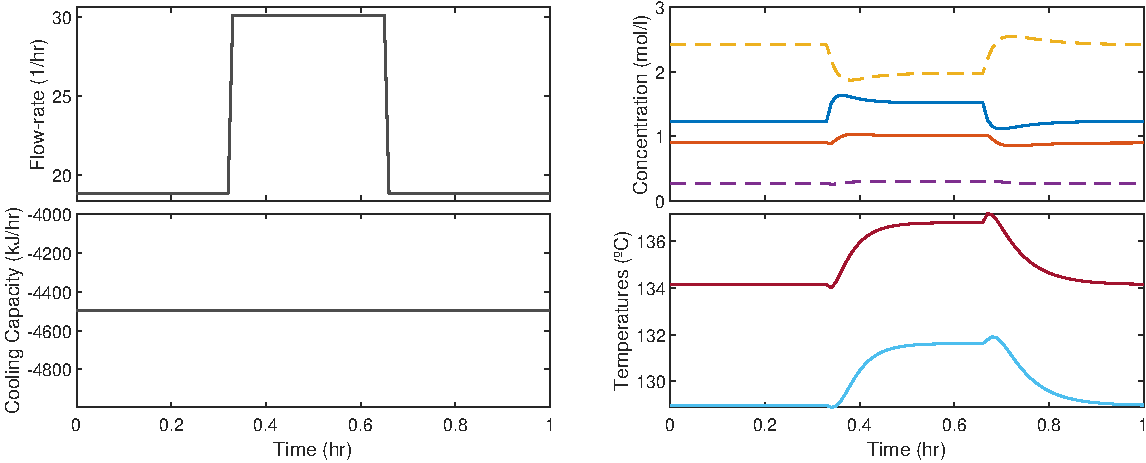
\includegraphics[width=\textwidth]{dynamics01}};
		
		\begin{scope}[on background layer]
			\node[block, minimum height=1.75em, above of=plot, xshift=0.41cm, node distance=2.75cm, minimum width=0.93\textwidth] (legendBox) {};
		\end{scope}
		
		\definecolor{linecolor}{rgb}{0, 0.4470, 0.7410};
		\node at (legendBox.west) [xshift=0.4cm]  (legendStart) {};
		\node[right of=legendStart, node distance=1cm] (label) {$\rho_A$};		
		\draw[-, linecolor, line width=1pt] (legendStart) -- (label);
		
		\definecolor{linecolor}{rgb}{0.8500,0.3250,0.0980};
		\node[right of=label]  (legendStart) {};
		\node[right of=legendStart, node distance=1cm] (label) {$\rho_B$};		
		\draw[-, linecolor, line width=1pt] (legendStart) -- (label);
		
		\definecolor{linecolor}{rgb}{0.9290, 0.6940, 0.1250};
		\node[right of=label]  (legendStart) {};
		\node[right of=legendStart, node distance=1cm] (label) {$\rho_C$};		
		\draw[-, dashed, linecolor, line width=1pt] (legendStart) -- (label);
		
		\definecolor{linecolor}{rgb}{0.4940, 0.1840, 0.5560};
		\node[right of=label]  (legendStart) {};
		\node[right of=legendStart, node distance=1cm] (label) {$\rho_D$};		
		\draw[-, dashed, linecolor, line width=1pt] (legendStart) -- (label);
		
		\definecolor{linecolor}{rgb}{0.6350, 0.0780, 0.1840};
		\node[right of=label]  (legendStart) {};
		\node[right of=legendStart, node distance=1cm] (label) {$T$};		
		\draw[-, linecolor, line width=1pt] (legendStart) -- (label);
		
		\definecolor{linecolor}{rgb}{0.3010, 0.7450, 0.9330};
		\node[right of=label]  (legendStart) {};
		\node[right of=legendStart, node distance=1cm] (label) {$T_c$};		
		\draw[-, linecolor, line width=1pt] (legendStart) -- (label);
	\end{tikzpicture}	
\end{figure}

\end{frame}

%-------------------------------------------------------
\begin{frame}[c]{Dynamical System Analysis}{Experiments}

\vskip0.25cm

\begin{figure}[ht] \centering
		\begin{tikzpicture}	[node distance=0.7cm]
		\node (plot) {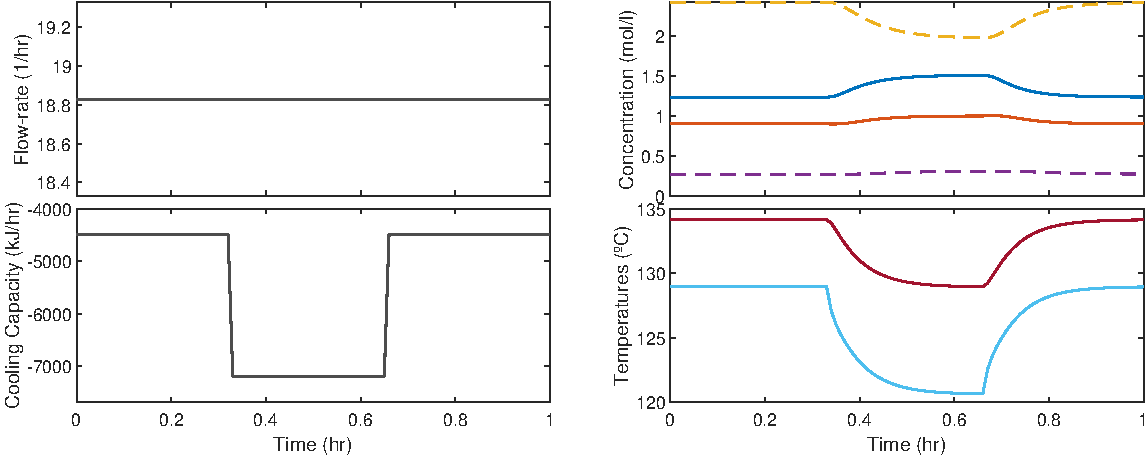
\includegraphics[width=\textwidth]{dynamics02}};
		
		\begin{scope}[on background layer]
			\node[block, minimum height=1.75em, above of=plot, xshift=0.41cm, node distance=2.75cm, minimum width=0.93\textwidth] (legendBox) {};
		\end{scope}
		
		\definecolor{linecolor}{rgb}{0, 0.4470, 0.7410};
		\node at (legendBox.west) [xshift=0.4cm]  (legendStart) {};
		\node[right of=legendStart, node distance=1cm] (label) {$\rho_A$};		
		\draw[-, linecolor, line width=1pt] (legendStart) -- (label);
		
		\definecolor{linecolor}{rgb}{0.8500,0.3250,0.0980};
		\node[right of=label]  (legendStart) {};
		\node[right of=legendStart, node distance=1cm] (label) {$\rho_B$};		
		\draw[-, linecolor, line width=1pt] (legendStart) -- (label);
		
		\definecolor{linecolor}{rgb}{0.9290, 0.6940, 0.1250};
		\node[right of=label]  (legendStart) {};
		\node[right of=legendStart, node distance=1cm] (label) {$\rho_C$};		
		\draw[-, dashed, linecolor, line width=1pt] (legendStart) -- (label);
		
		\definecolor{linecolor}{rgb}{0.4940, 0.1840, 0.5560};
		\node[right of=label]  (legendStart) {};
		\node[right of=legendStart, node distance=1cm] (label) {$\rho_D$};		
		\draw[-, dashed, linecolor, line width=1pt] (legendStart) -- (label);
		
		\definecolor{linecolor}{rgb}{0.6350, 0.0780, 0.1840};
		\node[right of=label]  (legendStart) {};
		\node[right of=legendStart, node distance=1cm] (label) {$T$};		
		\draw[-, linecolor, line width=1pt] (legendStart) -- (label);
		
		\definecolor{linecolor}{rgb}{0.3010, 0.7450, 0.9330};
		\node[right of=label]  (legendStart) {};
		\node[right of=legendStart, node distance=1cm] (label) {$T_c$};		
		\draw[-, linecolor, line width=1pt] (legendStart) -- (label);
	\end{tikzpicture}	
\end{figure}

\end{frame}

%-------------------------------------------------------
\begin{frame}[c]{Dynamical System Analysis}{Experiments}

\vskip0.25cm

\begin{figure}[ht] \centering
		\begin{tikzpicture}	[node distance=0.7cm]
		\node (plot) {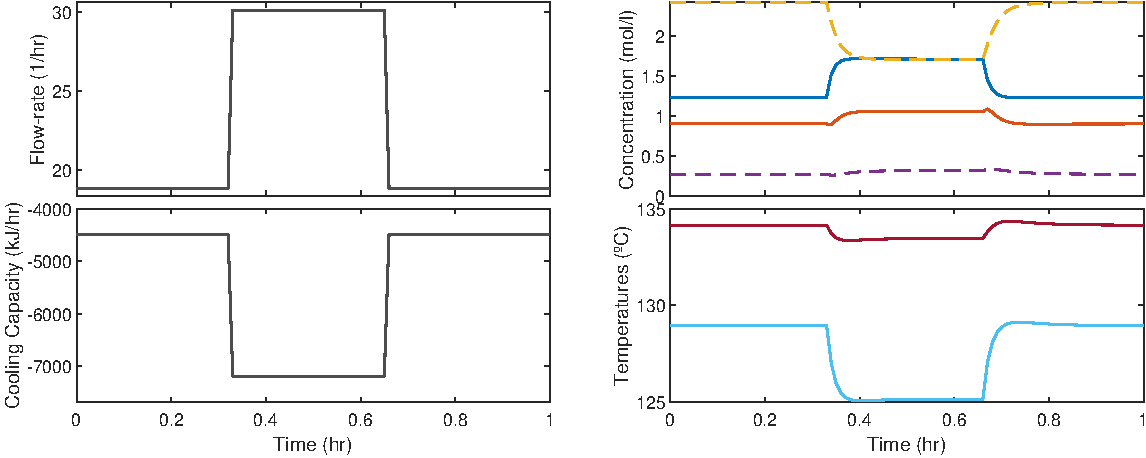
\includegraphics[width=\textwidth]{dynamics03}};
		
		\begin{scope}[on background layer]
			\node[block, minimum height=1.75em, above of=plot, xshift=0.41cm, node distance=2.75cm, minimum width=0.93\textwidth] (legendBox) {};
		\end{scope}
		
		\definecolor{linecolor}{rgb}{0, 0.4470, 0.7410};
		\node at (legendBox.west) [xshift=0.4cm]  (legendStart) {};
		\node[right of=legendStart, node distance=1cm] (label) {$\rho_A$};		
		\draw[-, linecolor, line width=1pt] (legendStart) -- (label);
		
		\definecolor{linecolor}{rgb}{0.8500,0.3250,0.0980};
		\node[right of=label]  (legendStart) {};
		\node[right of=legendStart, node distance=1cm] (label) {$\rho_B$};		
		\draw[-, linecolor, line width=1pt] (legendStart) -- (label);
		
		\definecolor{linecolor}{rgb}{0.9290, 0.6940, 0.1250};
		\node[right of=label]  (legendStart) {};
		\node[right of=legendStart, node distance=1cm] (label) {$\rho_C$};		
		\draw[-, dashed, linecolor, line width=1pt] (legendStart) -- (label);
		
		\definecolor{linecolor}{rgb}{0.4940, 0.1840, 0.5560};
		\node[right of=label]  (legendStart) {};
		\node[right of=legendStart, node distance=1cm] (label) {$\rho_D$};		
		\draw[-, dashed, linecolor, line width=1pt] (legendStart) -- (label);
		
		\definecolor{linecolor}{rgb}{0.6350, 0.0780, 0.1840};
		\node[right of=label]  (legendStart) {};
		\node[right of=legendStart, node distance=1cm] (label) {$T$};		
		\draw[-, linecolor, line width=1pt] (legendStart) -- (label);
		
		\definecolor{linecolor}{rgb}{0.3010, 0.7450, 0.9330};
		\node[right of=label]  (legendStart) {};
		\node[right of=legendStart, node distance=1cm] (label) {$T_c$};		
		\draw[-, linecolor, line width=1pt] (legendStart) -- (label);
	\end{tikzpicture}	
\end{figure}

\end{frame}

%-------------------------------------------------------
\begin{frame}[c]{Dynamical System Analysis}{Experiments}

\vskip0.25cm

\begin{figure}[ht] \centering
		\begin{tikzpicture}	[node distance=1cm]
		\node (plot) {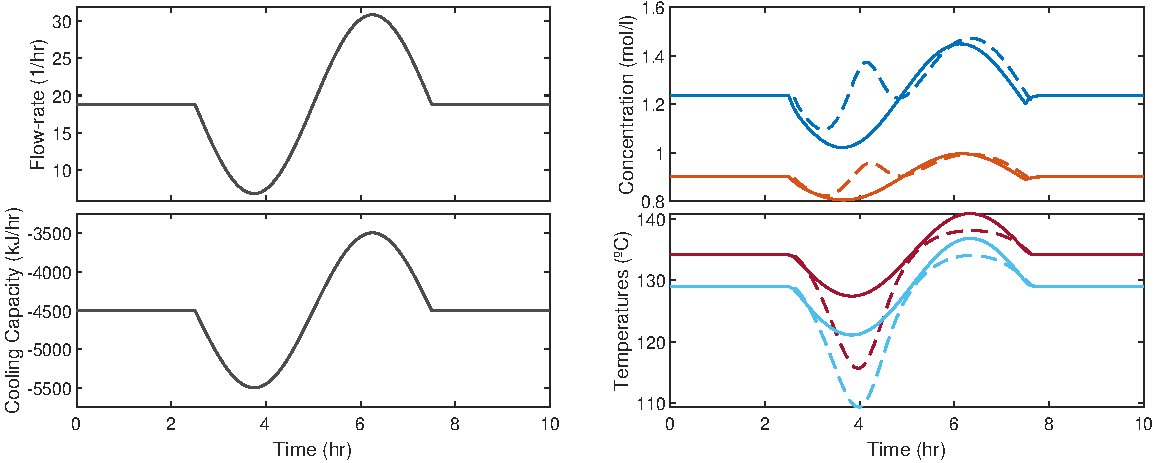
\includegraphics[width=\textwidth]{linear01}};
		
		\begin{scope}[on background layer]
			\node[block, minimum height=1.75em, above of=plot, xshift=0.45cm, node distance=2.75cm, minimum width=0.7\textwidth] (legendBox) {};
		\end{scope}
		
		\definecolor{linecolor}{rgb}{0, 0.4470, 0.7410};
		\node at (legendBox.west) [xshift=0.4cm]  (legendStart) {};
		\node[right of=legendStart, node distance=1cm] (label) {$\rho_A$};		
		\draw[-, linecolor, line width=1pt] (legendStart) -- (label);
		
		\definecolor{linecolor}{rgb}{0.8500,0.3250,0.0980};
		\node[right of=label]  (legendStart) {};
		\node[right of=legendStart, node distance=1cm] (label) {$\rho_B$};		
		\draw[-, linecolor, line width=1pt] (legendStart) -- (label);
		
		\definecolor{linecolor}{rgb}{0.6350, 0.0780, 0.1840};
		\node[right of=label]  (legendStart) {};
		\node[right of=legendStart, node distance=1cm] (label) {$T$};		
		\draw[-, linecolor, line width=1pt] (legendStart) -- (label);
		
		\definecolor{linecolor}{rgb}{0.3010, 0.7450, 0.9330};
		\node[right of=label]  (legendStart) {};
		\node[right of=legendStart, node distance=1cm] (label) {$T_c$};		
		\draw[-, linecolor, line width=1pt] (legendStart) -- (label);
	\end{tikzpicture}	
\end{figure}

\end{frame}

%-------------------------------------------------------
% SECTION - State-Feedback Controllers
%-------------------------------------------------------
\section{State-Feedback Controllers}
%-------------------------------------------------------
\subsection{Definitions}
%-------------------------------------------------------
\begin{frame}[t]{State-Feedback Controllers}{Definitions}

\vskip0.25cm

\begin{varblock}[1\linewidth]{Full State-Feedback Controller}
	    Given a linear system in State-Space representation, an input action $\bm{u}(t)$ is calculated by the linear control law $\pi(\cdot)$ through state-feedback as:
    \begin{equation}
        \bm{u}(t) = \pi(\bm{r}(t), \bm{x}(t)) = \bm{r}(t) - \bm{K} \bm{x}(t)
    ,\end{equation}
    
    \noindent where $\bm{r} : \mathbb{R} \rightarrow \mathbb{R}^{n}$ is a state reference signal that the system must follows and $\bm{K} \in \mathbb{R}^{r \times n}$ is the \textit{feedback gain matrix}.
\end{varblock}

\end{frame}

%-------------------------------------------------------
\begin{frame}[t]{State-Feedback Controllers}{Definitions}

\vskip0.25cm

\begin{varblock}[1\linewidth]{Full State-Feedback Controller}
	Given a linear system in State-Space representation, an input action $\bm{u}(t)$ is calculated by the linear control law $\pi(\cdot)$ through state-feedback as:
    \begin{equation}
        \bm{u}(t) = \pi(\bm{r}(t), \bm{x}(t)) = \bm{r}(t) - \bm{K} \bm{x}(t)
    ,\end{equation}
    
    \noindent where $\bm{r} : \mathbb{R} \rightarrow \mathbb{R}^{n}$ is a state reference signal that the system must follows and $\bm{K} \in \mathbb{R}^{r \times n}$ is the \textit{feedback gain matrix}.
\end{varblock}

\begin{varblock}[1\linewidth]{Pole-Placement Property}
	If a system in State-Space representation is controllable, then by state feedback using a gain matrix $\bm{K} \in \mathbb{R}^{r \times n}$ the eigenvalues of $\bm{A}_{cl}=\bm{A}-\bm{B}\bm{K}$, the poles of the closed-loop system, can be placed arbitrarily in the complex plane, as long as complex conjugate eigenvalues are assigned in pairs.
\end{varblock}

\end{frame}

%-------------------------------------------------------
\begin{frame}[c]{State-Feedback Controllers}{Definitions}

\vskip0.25cm

\begin{figure}[ht]
    \centering
    \resizebox{!}{!}{
    \begin{tikzpicture}[auto, node distance=2cm,>=latex', scale=0.2]
        % We start by placing the blocks
        \node [input, name=input] {};
        \node [sum, right of=input, node distance=4em] (fbckSum) {};
        \node [block, right of=fbckSum] (inputMatrix) {$\bm{B}$};
        \node [sum, right of=inputMatrix, node distance=4em] (stateSum) {};
        \node [block, right of=stateSum, node distance=4em] (integral) {$\int   $};
        \node [block, right of=integral, node distance=8em] (outputMatrix) {$\bm{C}$};
        \node [output, right of=outputMatrix] (output) {};
        \node [block, below of=integral, node distance=1.5cm] (stateMatrix) {$\bm{A}$};
        \node [block, below of=stateSum, node distance=11em, label={below:Controller}] (fbckGain) {$\bm{K}$};
        
        \begin{scope}[on background layer]
            \node [fit=(inputMatrix) (stateMatrix) (outputMatrix), fill= glgBlue!10, rounded corners, inner sep=.4cm, label={[xshift=3.5em, glgBlue!90]above left:Open-Loop System}] {};
        \end{scope}     
        
        % Once the nodes are placed, connecting them is easy.       
        \draw [draw,->] (input) -- node[pos=0.1] {$\bm{r}$} node[pos=0.8] {$+$}  (fbckSum);
        \draw [->] (fbckSum) -- node[pos=0.3]{$\bm{u}$} (inputMatrix);
        \draw [->] (inputMatrix) -- node[pos=0.8]{$+$} (stateSum);
        \draw [->] (stateSum) -- node[pos=0.5]{$\dot{\bm{x}}$} (integral);
        \draw [->] (integral) -- node[name=bk1,pos=0.5]{} node[name=bk2,pos=0.5]{} node[pos=0.5]{$\bm{x}$} (outputMatrix);
        \draw [->] (outputMatrix) -- node[pos=0.6]{$\bm{y}$} (output);
        \draw [->] (bk1) |- (stateMatrix);
        \draw [->] (bk2) |- (fbckGain);
        \draw [->] (stateMatrix) -| node[pos=0.95]{$+$} (stateSum);
        \draw [->] (fbckGain) -| node[pos=0.97]{$-$} (fbckSum);
    \end{tikzpicture} 
    }
\end{figure}

\end{frame}

%-------------------------------------------------------
\subsection{Regulation vs. Tracking}
%-------------------------------------------------------
\begin{frame}[t]{State-Feedback Controllers}{Regulation vs. Tracking}

\vskip0.25cm
{\justifying During the semester, we have discussed Conservation Laws of fluid elements...}


\begin{varblock}[1\linewidth]{Conservation of Mass}
	\begin{equation*}
		{\begin{pmatrix}
			\text{Time rate of} \\
			\text{change of mass} \\
			\text{in the system}
		\end{pmatrix}} = 
		{\begin{pmatrix}
			\text{Mass} \\
			\text{entering} \\
			\text{the system}
		\end{pmatrix}} - 
		{\begin{pmatrix}
			\text{Mass} \\
			\text{leaving} \\
			\text{the system}
		\end{pmatrix}}
	\end{equation*} \vskip0.2cm
\end{varblock}

\end{frame}

%-------------------------------------------------------
\begin{frame}[c]{State-Feedback Controllers}{Regulation vs. Tracking}

\vskip0.25cm

\begin{figure}[ht]
    \centering
    \resizebox{\textwidth}{!}{
    \begin{tikzpicture}[auto, node distance=2cm,>=latex']
        % We start by placing the blocks
        \node [input, name=input] {};
        \node [sum, right of=input, node distance=4em] (intFbckSum) {};
        \node [block, right of=intFbckSum, node distance=4em] (integralAction) {$\int$};
        \node [block, right of=integralAction, node distance=6em] (intActGain) {$\bm{K}_a$};
        \node [sum, right of=intActGain, node distance=4.5em] (fbckSum) {};
        \node [block, right of=fbckSum] (inputMatrix) {$\bm{B}$};
        \node [sum, right of=inputMatrix, node distance=4em] (stateSum) {};
        \node [block, right of=stateSum, node distance=4em] (integral) {$\int   $};
        \node [block, right of=integral, node distance=8em] (outputMatrix) {$\bm{C}$};
        \node [output, right of=outputMatrix] (output) {};
        \node [block, below of=integral] (stateMatrix) {$\bm{A}$};
        \node [block, below of=stateSum, node distance=13em, label={below:Controller}] (fbckGain) {$\bm{K}$};
        
        \begin{scope}[on background layer]
            \node [fit=(inputMatrix) (stateMatrix) (outputMatrix), fill= glgBlue!10, rounded corners, inner sep=.4cm, label={[xshift=3.5em, glgBlue!90]above left:Open-Loop System}] {};
        \end{scope}     
        
        \begin{scope}[on background layer]
            \node [fit=(integralAction) (intActGain), fill= glgGreen!10, rounded corners, inner sep=.4cm, label={[xshift=4.3em, glgGreen!90]above left:Integral Action}] {};
        \end{scope} 
        
        % Once the nodes are placed, connecting them is easy.       
        \draw [draw,->] (input) -- node[pos=0.1] {$\bm{r}$} node[pos=0.8] {$+$}  (intFbckSum);
        \draw [->] (intFbckSum) -- (integralAction);
        \draw [->] (integralAction) -- node[pos=0.5]{$\bm{x}_a$} (intActGain);
        \draw [->] (intActGain) -- node[pos=0.8]{$-$} (fbckSum);
        \draw [->] (fbckSum) -- node[pos=0.3]{$\bm{u}$} (inputMatrix);
        \draw [->] (inputMatrix) -- node[pos=0.8]{$+$} (stateSum);
        \draw [->] (stateSum) -- node[pos=0.5]{$\dot{\bm{x}}$} (integral);
        \draw [->] (integral) -- node[name=bk1,pos=0.5]{} node[name=bk2,pos=0.5]{} node[pos=0.5]{$\bm{x}$} (outputMatrix);
        \draw [->] (outputMatrix) -- node[name=bk3,pos=0.5]{} node[pos=0.6]{$\bm{y}$} (output);
        \draw [->] (bk1) |- (stateMatrix);
        \draw [->] (bk2) |- (fbckGain);
        \draw [->] (stateMatrix) -| node[pos=0.95]{$+$} (stateSum);
        \draw [->] (fbckGain) -| node[pos=0.97]{$-$} (fbckSum);
        \draw [->] (bk3) -- ++(0, -17em) -| node[pos=0.97]{$-$} (intFbckSum);
    \end{tikzpicture} 
    }
\end{figure}

\end{frame}

%-------------------------------------------------------
% SECTION - Optimal Control
%-------------------------------------------------------
\section{Optimal Control}
%-------------------------------------------------------
\subsection{Formulation}
%-------------------------------------------------------
\begin{frame}[t]{Optimal Control}{Formulation}

\vskip0.25cm

\begin{varblock}[1\linewidth]{Optimal Controller}
	Given a system in State-Space formulation, with state signal $\bm{x} : \mathbb{R} \rightarrow \mathbb{R}^{n}$, and a reference signal $\bm{r} : \mathbb{R} \rightarrow \mathbb{R}^{n}$, the input signal $\bm{u}	(t) \in \mathbb{R}^r$, for any time $t$, is optimal if an optimal control law $\pi^* : \mathbb{R}^{n \times n \times 1} \rightarrow \mathbb{R}^r$ can be found as:
	    \begin{equation}
	        \bm{u}(t) = \pi^*(\bm{x}, \bm{r}, t) = \min_{\bm{u}} J(\bm{x}, \bm{r}, t)
	    ,\end{equation}
	    
	\noindent where $J : \mathbb{R}^{n \times n \times 1} \rightarrow \mathbb{R}$ is known as a \textit{cost function} of the states and reference signals.
\end{varblock}

\end{frame}

%-------------------------------------------------------
\begin{frame}[t]{Optimal Control}{Formulation}

\vskip0.25cm

\begin{varblock}[1\linewidth]{Optimal Controller}
	Given a system in State-Space formulation, with state signal $\bm{x} : \mathbb{R} \rightarrow \mathbb{R}^{n}$, and a reference signal $\bm{r} : \mathbb{R} \rightarrow \mathbb{R}^{n}$, the input signal $\bm{u}	(t) \in \mathbb{R}^r$, for any time $t$, is optimal if an optimal control law $\pi^* : \mathbb{R}^{n \times n \times 1} \rightarrow \mathbb{R}^r$ can be found as:
	    \begin{equation}
	        \bm{u}(t) = \pi^*(\bm{x}, \bm{r}, t) = \min_{\bm{u}} J(\bm{x}, \bm{r}, t)
	    ,\end{equation}
	    
	\noindent where $J : \mathbb{R}^{n \times n \times 1} \rightarrow \mathbb{R}$ is known as a \textit{cost function} of the states and reference signals.
\end{varblock}

\begin{varblock}[1\linewidth]{Finite-Horizon Optimal Regulators}
	A \textit{Finite-Horizon Optimal Regulator} is defined as any controller whose optimal policy over a time interval $t \in [t_0, T]$ minimizes the cost functional:
    \begin{equation}
        J(\bm{x}, \bm{u}, t_0) = \int_{t_0}^T l(\bm{x}, \bm{u}, \tau) d \tau + l_f(\bm{x}, T)
    ,\end{equation}
    
    \noindent where $l(\cdot) : \mathbb{R}^{n \times r \times 1} \rightarrow \mathbb{R}$ and $l_f(\cdot) : \mathbb{R}^{n} \rightarrow \mathbb{R}$ are, respectively, the \textit{trajectory} and \textit{terminal loss functions}. In the case that $t_0 = 0$, $T$ is also known as the \textit{control horizon}.
\end{varblock}

\end{frame}

%-------------------------------------------------------
\begin{frame}[t]{Optimal Control}{Formulation}

\vskip0.25cm

\begin{varblock}[1\linewidth]{Hamilton-Jacobi-Bellman Equation}
	Consider a finite-horizon cost function for a system described by $\dot{\bm{x}} = \bm{f}(\bm{x}, \bm{u}, t)$:
    \begin{equation} \label{eq:valueCostFunctional}
    	V(\bm{x}, \bm{u}, t_0) = \int_{t_0}^T l(\bm{x}, \bm{u}, \tau) d \tau + l_f(\bm{x}(T))
    \end{equation}
    
    \noindent Consider also that the loss $l(\cdot)$ and state function $\bm{f}$ are smooth on their parameters. Then, minimizing any functional in the form of $V(\cdot)$ is equivalent to determining the solution of the \textit{Hamilton-Jacobi equation}, which is given by the partial differential equation:
    \begin{equation} \label{eq:HJEquation}
        \cfrac{\partial V^*}{\partial t} = - \min_{u(t)} \left[ l(\bm{x}, \bm{u}, t) + \left[ \cfrac{\partial V^*}{\partial x} \right]^T \bm{f}(\bm{x}, \bm{u}, t)  \right]
    \end{equation}
    
    \noindent and the boundary condition:
    \begin{equation}
        V^*(\bm{x}, T) = l_f(\bm{x}(T))
    .\end{equation} \vskip0.2cm
\end{varblock}

\end{frame}

%-------------------------------------------------------
\begin{frame}[c]{Optimal Control}{Formulation}

\vskip0.25cm

\begin{figure}[ht] \centering
    \resizebox{!}{!}{
    \begin{tikzpicture}[auto, node distance=1.75cm,>=latex', scale=0.2]
        % Nodes
        \node [mcCircle] (x0) {$x_0$};
        
        \node [mcCircle, right of=x0, node distance=12em] (x12) {};
        \node [mcCircle, above of=x12] (x11) {};
        \node [mcCircle, below of=x12] (x13) {};
        
        \node [mcCircle, right of=x12, node distance=14em] (xT) {$x_T$};
        
        % Scopes
        \begin{scope}[on background layer]
            \node [fit=(x11) (x13), fill= black!10, rounded corners, inner sep=.4cm, label={[xshift=0em, black!90]above:$x_1$}] {};
        \end{scope}         
        
        % Lines
        \draw [->, color=glgRed!80, line width=.75mm] (x0) -- node[pos=0.7]{$70$} (x11);
        \draw [->] (x0) -- node[pos=0.6]{$40$} (x12);
        \draw [->] (x0) -- node[pos=0.45]{$130$} (x13);
        
        \draw [->, color=glgRed!80, line width=.75mm, decorate, decoration={snake,amplitude=1.5mm, segment length=8mm}] (x11) -- node[pos=0.31]{$220$} (xT);
        \draw [->, decorate, decoration={snake,amplitude=1.5mm, segment length=8mm}] (x12) -- node[pos=0.48]{$270$} (xT);
        \draw [->, decorate, decoration={snake,amplitude=1.5mm, segment length=8mm}] (x13) -- node[pos=0.53]{$190$} (xT);
    \end{tikzpicture} 
    }
\end{figure}

\end{frame}


%-------------------------------------------------------
\subsection{Linear Quadratic (LQ) Controllers}
%-------------------------------------------------------
\begin{frame}[t]{Optimal Control}{Linear Quadratic (LQ) Controllers}

\vskip0.25cm

\begin{varblock}[1\linewidth]{Linear Quadratic Regulator (LQR)}
	Given a linear State-Space system in the form:
    \begin{align}
    \begin{cases}
        \dot{\bm{x}}(t) = \bm{A} \bm{x}(t) + \bm{B} \bm{u}(t) \\
        \bm{y}(t) = \bm{C} \bm{x}(t) + \bm{D} \bm{u}(t)
    \end{cases}
    .\end{align}
    
    A \textit{Linear Quadratic Regulator} (LQR) for this system is an optimal controller defined by the quadratic cost function:
    \begin{equation}
        J(\bm{x}, \bm{u}, t_0) = \int_{t_0}^{T} \left( \bm{x}^T \bm{Q} \bm{x} + \bm{u}^T \bm{R} \bm{u} \right) dt + \bm{x}^T(T) \bm{Q}_f \bm{x}(T)
    ,\end{equation}
    
    \noindent where is assumed that $\bm{Q},\bm{Q}_f  \succ 0$ and $\bm{R} \succ 0$ are matrices penalizing, respectively, the state-vector magnitude and the control effort.
\end{varblock}

\end{frame}

%-------------------------------------------------------
\begin{frame}[t]{Optimal Control}{Linear Quadratic (LQ) Controllers}

\vskip0.25cm

\begin{varblock}[1\linewidth]{LQR Control Action from Dynamic Programming}
	Given a Linear Quadratic Regulator, the optimal action produced by this optimal controller at any time $t \in [t_0, T]$ is given by:
    \begin{equation}
        \bm{u}^*(t) = - \bm{R}^{-1} \bm{B}^T \bm{P}(t) \bm{x}(t)
    ,\end{equation}
    
    \noindent where $\bm{P}(t)$ is the solution of the matrix Riccati differential equation:
    \begin{equation}
        -\dot{\bm{P}}(t) = \bm{A}^T \bm{P}(t) + \bm{P}(t) \bm{A} - \bm{P}(t) \bm{B} \bm{R}^{-1} \bm{B}^T \bm{P}(t) + \bm{Q}
    ,\end{equation}
    
    \noindent with terminal condition $\bm{P}(T) = \bm{Q}_f$.
\end{varblock}

\end{frame}

%-------------------------------------------------------
\begin{frame}[t]{Optimal Control}{Linear Quadratic (LQ) Controllers}

\vskip0.25cm

\begin{varblock}[1\linewidth]{LQR with Integral Action}
	Given a linear State-Space system represented by matrices $(\bm{A}, \bm{B}, \bm{C}, \bm{D})$, augmented with state $\dot{\bm{x}}_a(t) = \bm{r}(t) - \bm{C} \bm{x}(t)$:
    \begin{align} 
    \begin{cases}
        \begin{bmatrix}
            \dot{\bm{x}}(t) \\
            \dot{\bm{x}}_a(t)
        \end{bmatrix} &= \underbrace{\begin{bmatrix}
            \bm{A}  & \bm{0} \\ - \bm{C} & \bm{0}
        \end{bmatrix}}_{\tilde{\bm{A}}} \underbrace{\begin{bmatrix}
            \bm{x}(t) \\
            \bm{x}_a(t)
        \end{bmatrix}}_{\tilde{\bm{x}}(t)} + \underbrace{\begin{bmatrix}
            \bm{B} \\
            \bm{0}
        \end{bmatrix}}_{\tilde{\bm{B}}} \bm{u}(t) + \begin{bmatrix}
            \bm{0} \\
            \bm{I}
        \end{bmatrix} \bm{r}(t)
        \\
        \hfill \bm{y}(t) &= \begin{bmatrix}
            \bm{C} & \bm{0}
        \end{bmatrix} \begin{bmatrix}
            \bm{x}(t) \\
            \bm{x}_a(t)
        \end{bmatrix}
    \end{cases}
    .\end{align}
    
    A \textit{Linear Quadratic Servo} (LQ-Servo) for this system is an optimal controller defined by the quadratic cost function:
    \begin{equation}
        J(\bm{x}, \bm{u}, t_0) = \int_{t_0}^{T} \left( \tilde{\bm{x}}^T \tilde{\bm{Q}} \tilde{\bm{x}} + \bm{u}^T \bm{R} \bm{u} \right) dt +\tilde{\bm{x}} \tilde{\bm{Q}}_f \tilde{\bm{x}}(T)
    ,\end{equation}
    
    \noindent where is assumed that $\tilde{\bm{Q}}, \tilde{\bm{Q}}_f \succ 0$ and $\bm{R} \succ 0$ are matrices penalizing, respectively, the state-vector magnitude and the control effort.
\end{varblock}

\end{frame}

%-------------------------------------------------------
\subsection{Simulations}
%-------------------------------------------------------
\begin{frame}[c]{Optimal Control}{Simulations}

\vskip0.25cm

\begin{figure}[h]
	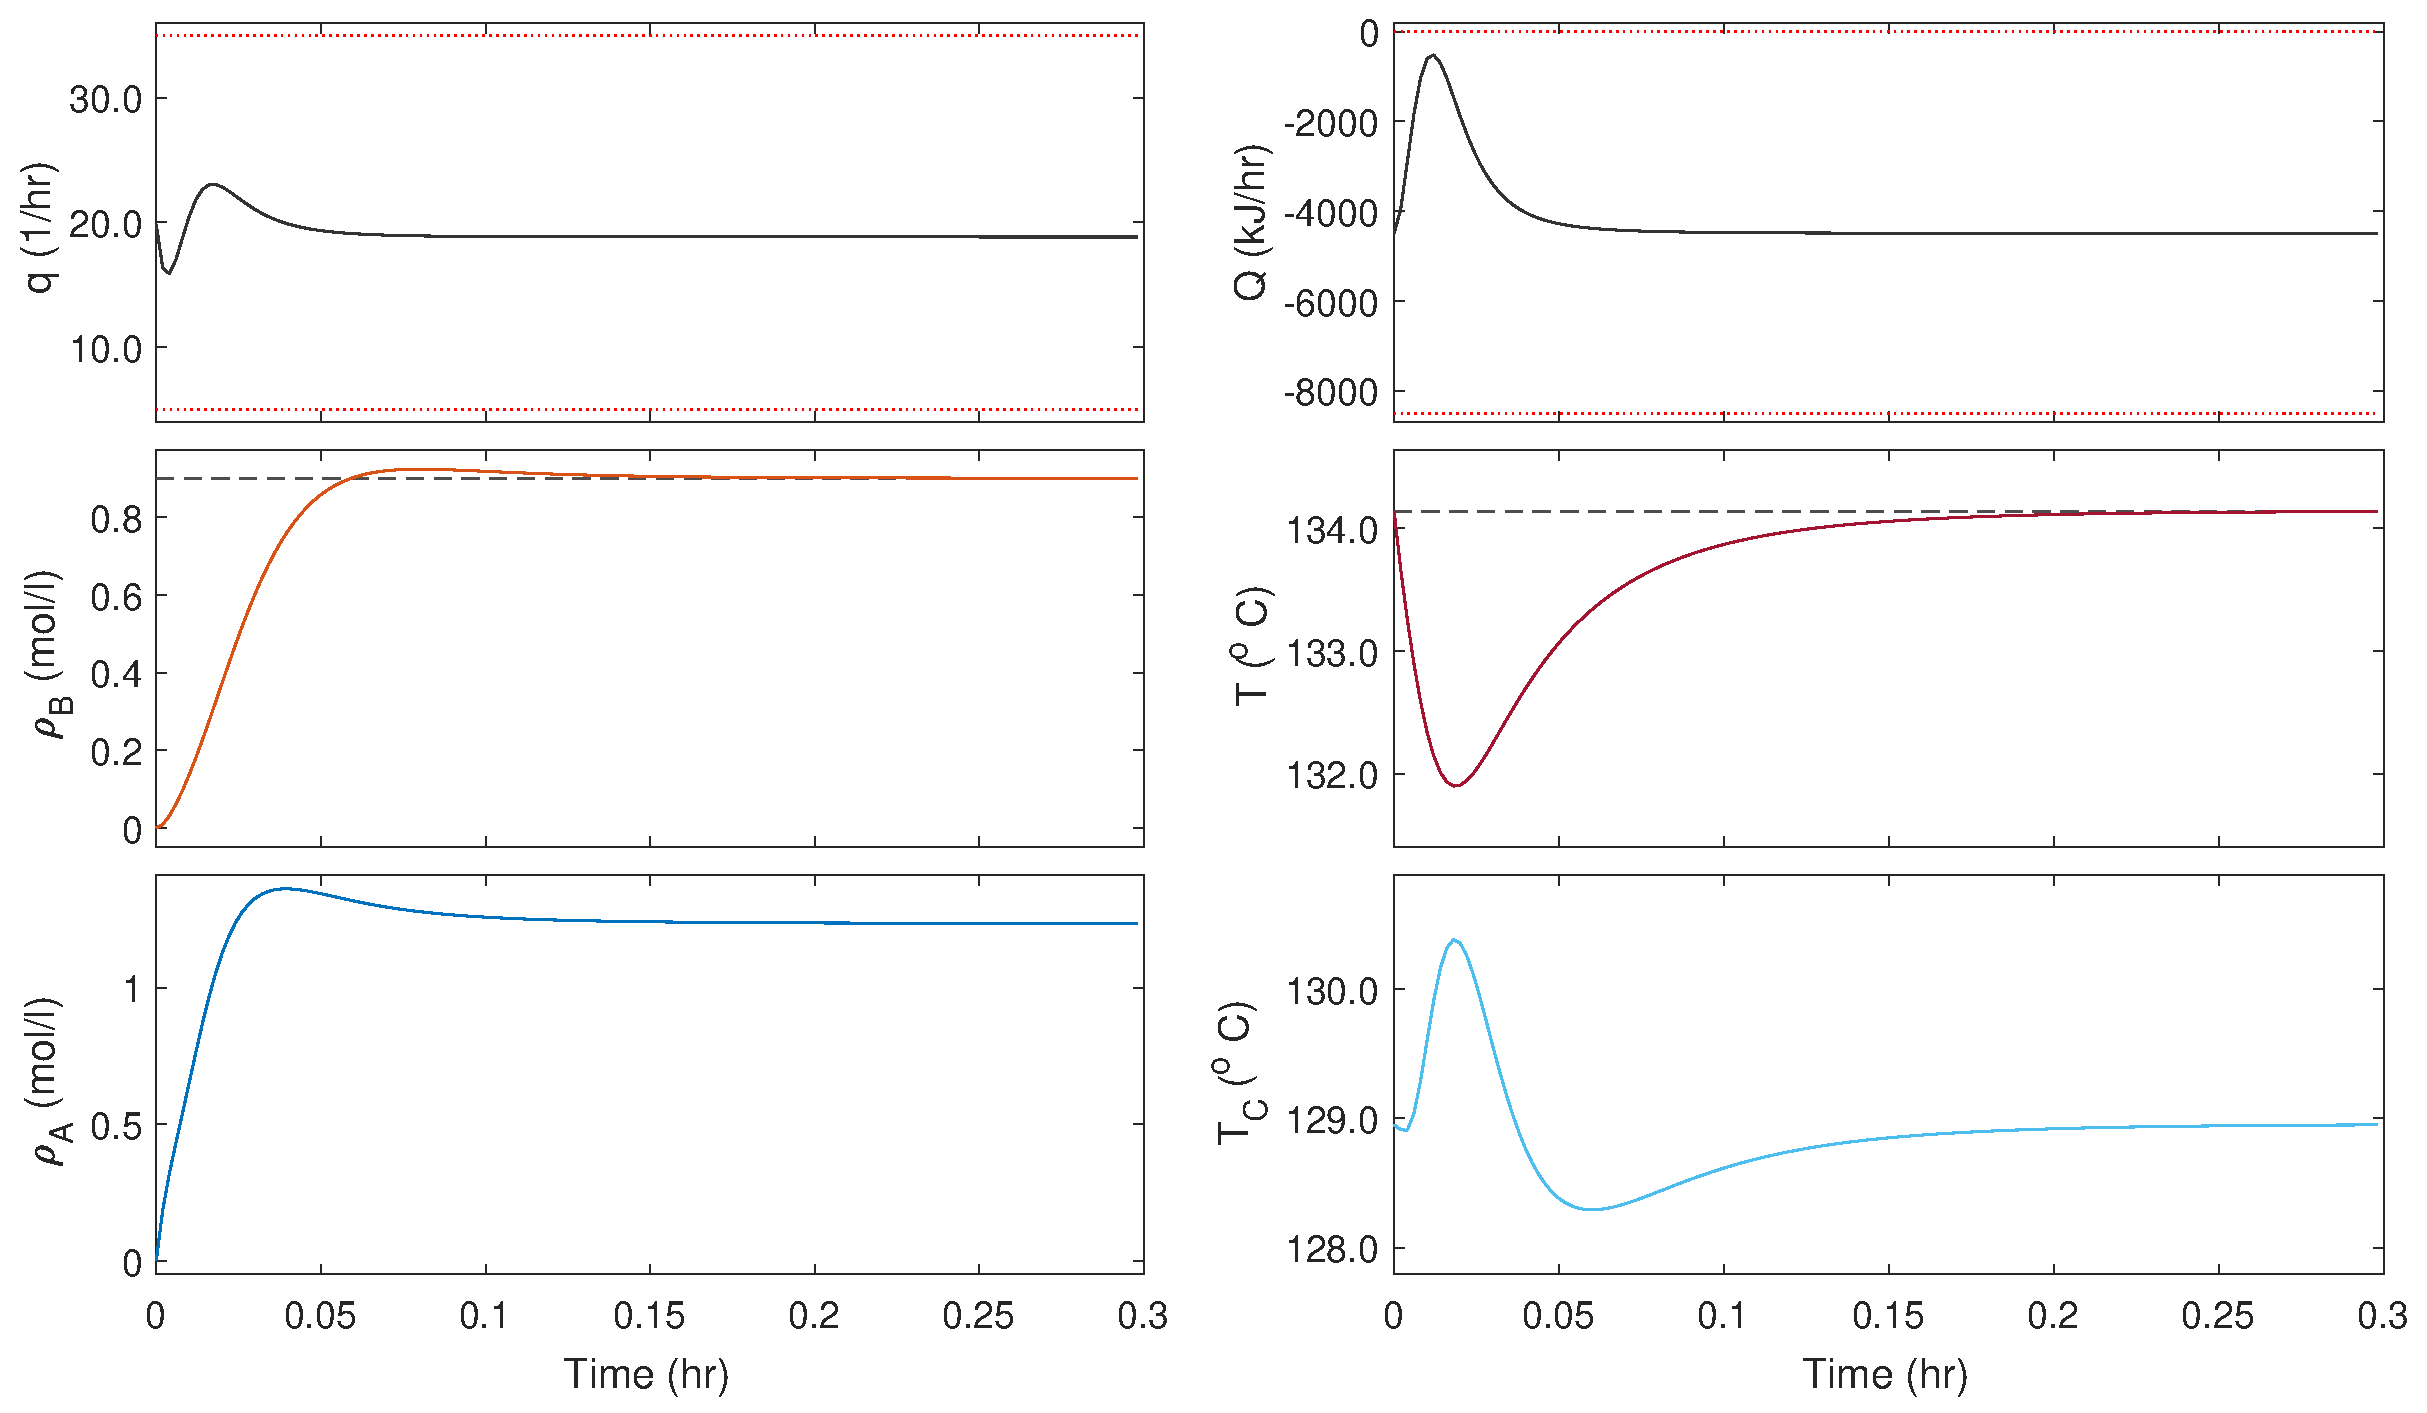
\includegraphics[width=\textwidth]{lqr01}
\end{figure}

\end{frame}

%-------------------------------------------------------
\begin{frame}[c]{Optimal Control}{Simulations}

\vskip0.25cm

\begin{figure}[h]
	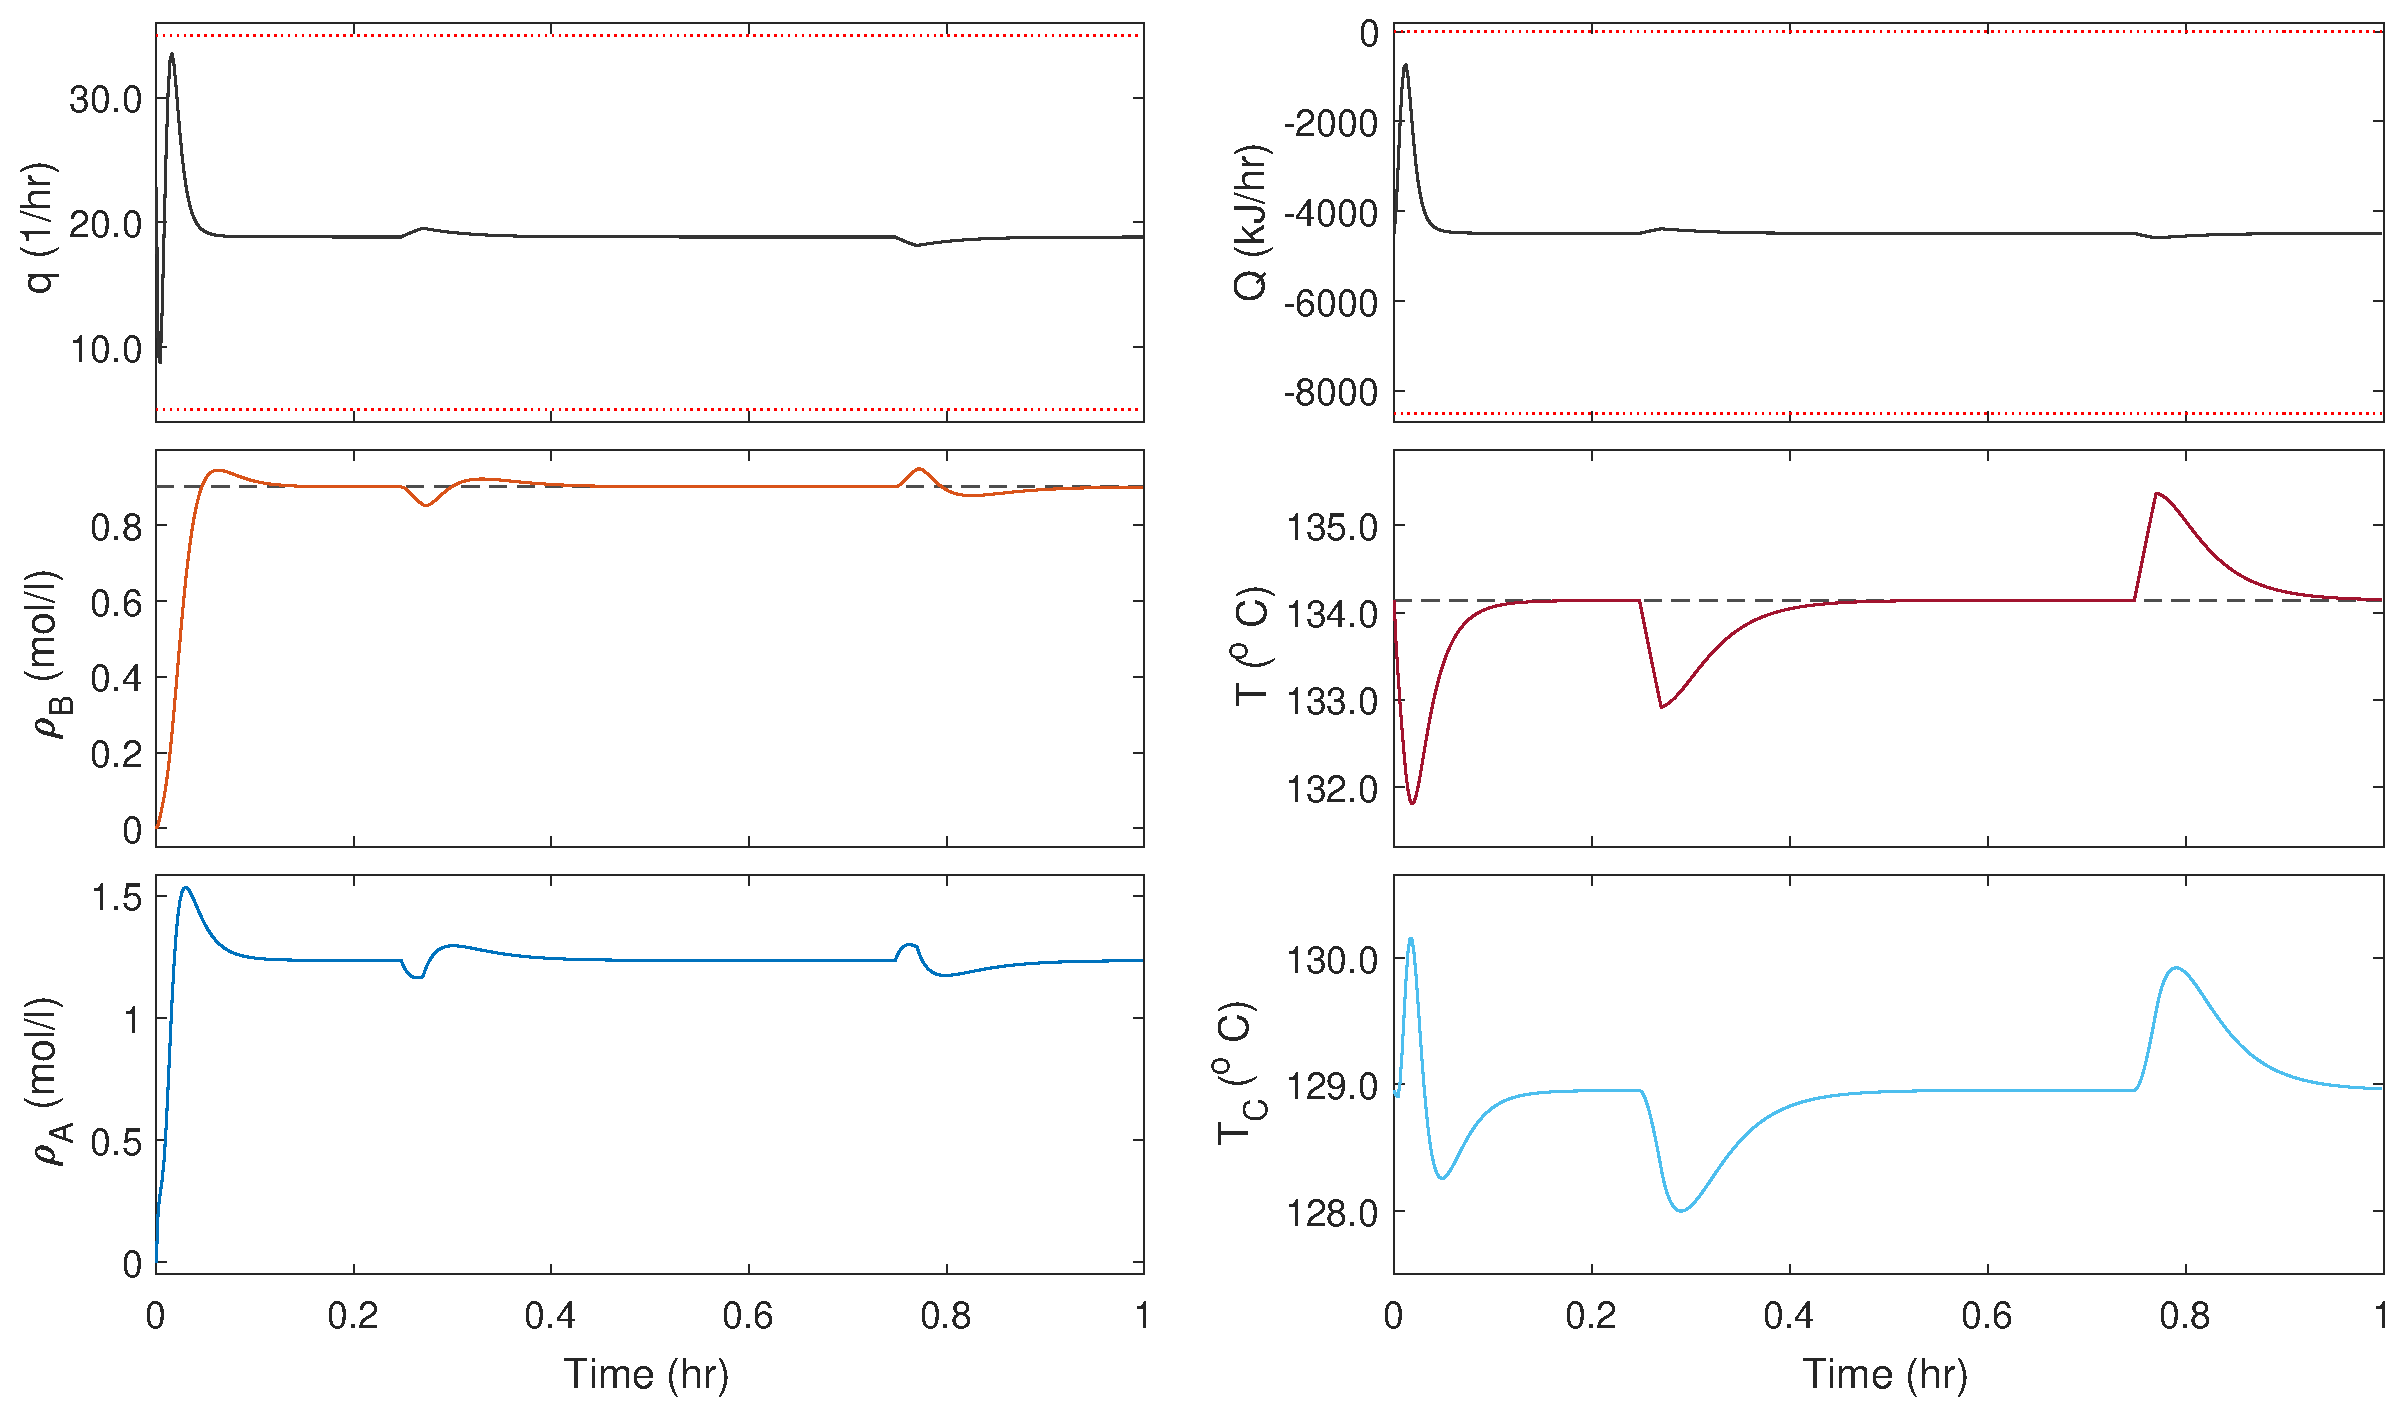
\includegraphics[width=\textwidth]{lqr02}
\end{figure}

\end{frame}

%-------------------------------------------------------
\begin{frame}[c]{Optimal Control}{Simulations}

\vskip0.25cm

\begin{figure}[h]
	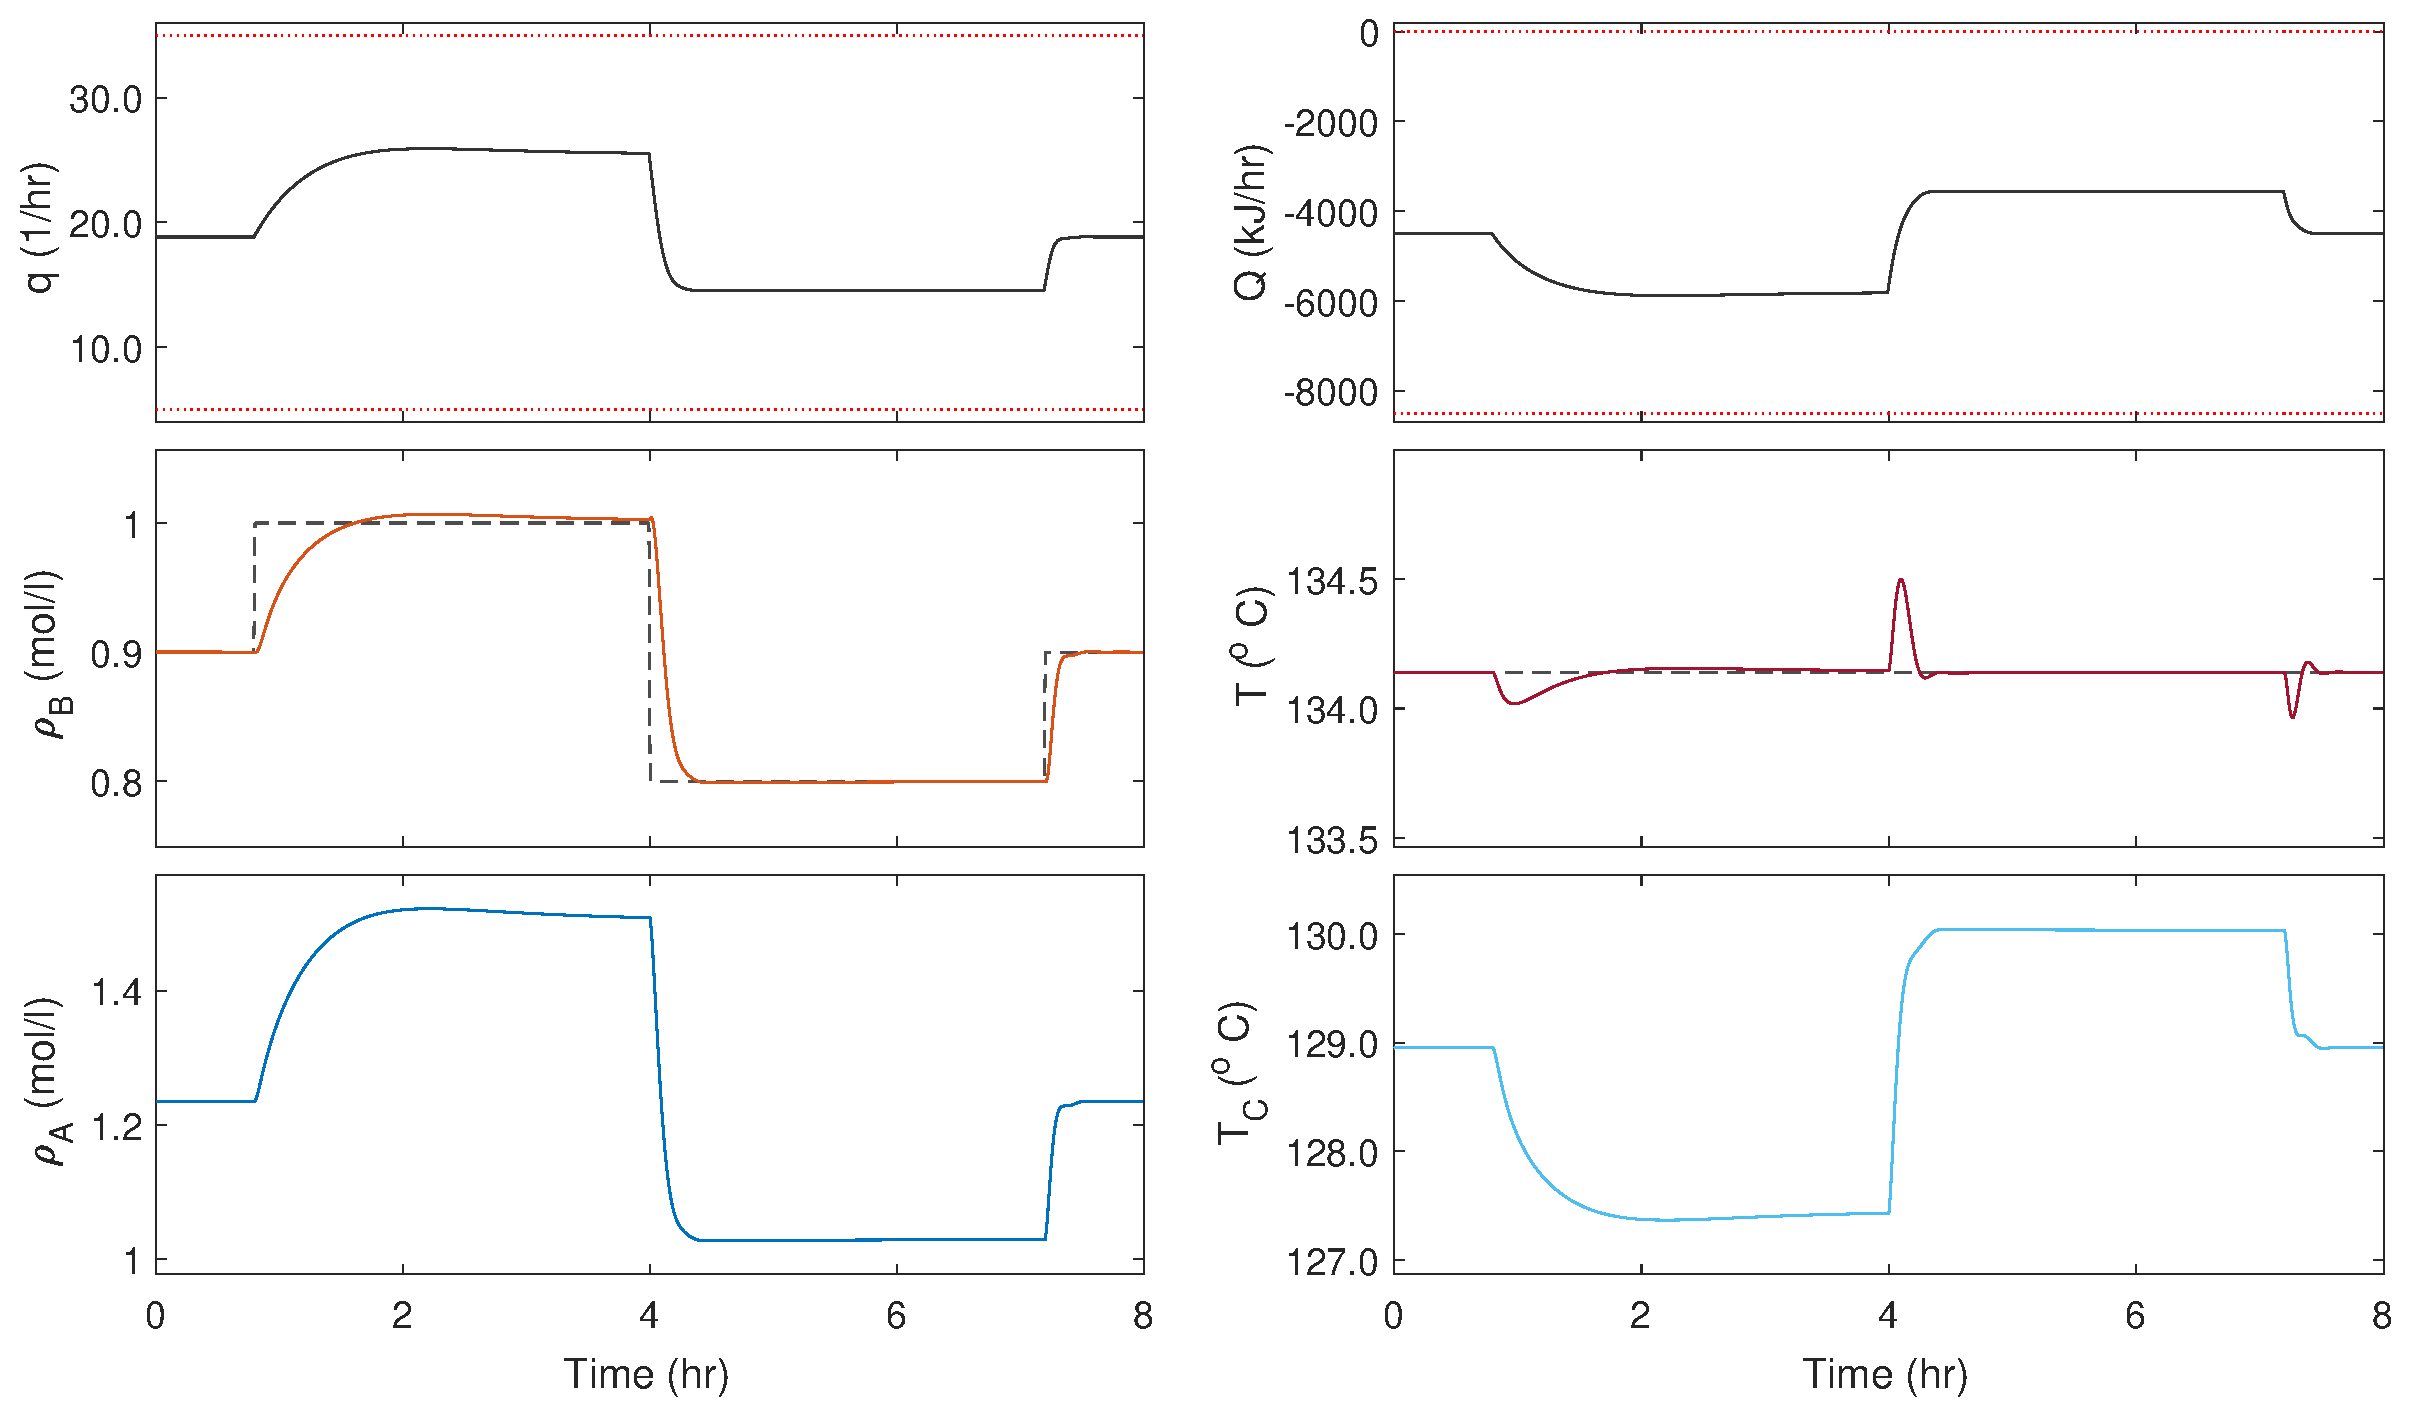
\includegraphics[width=\textwidth]{lqri01}
\end{figure}

\end{frame}

%-------------------------------------------------------
\begin{frame}[c]{Optimal Control}{Simulations}

\vskip0.25cm

\begin{figure}[h]
	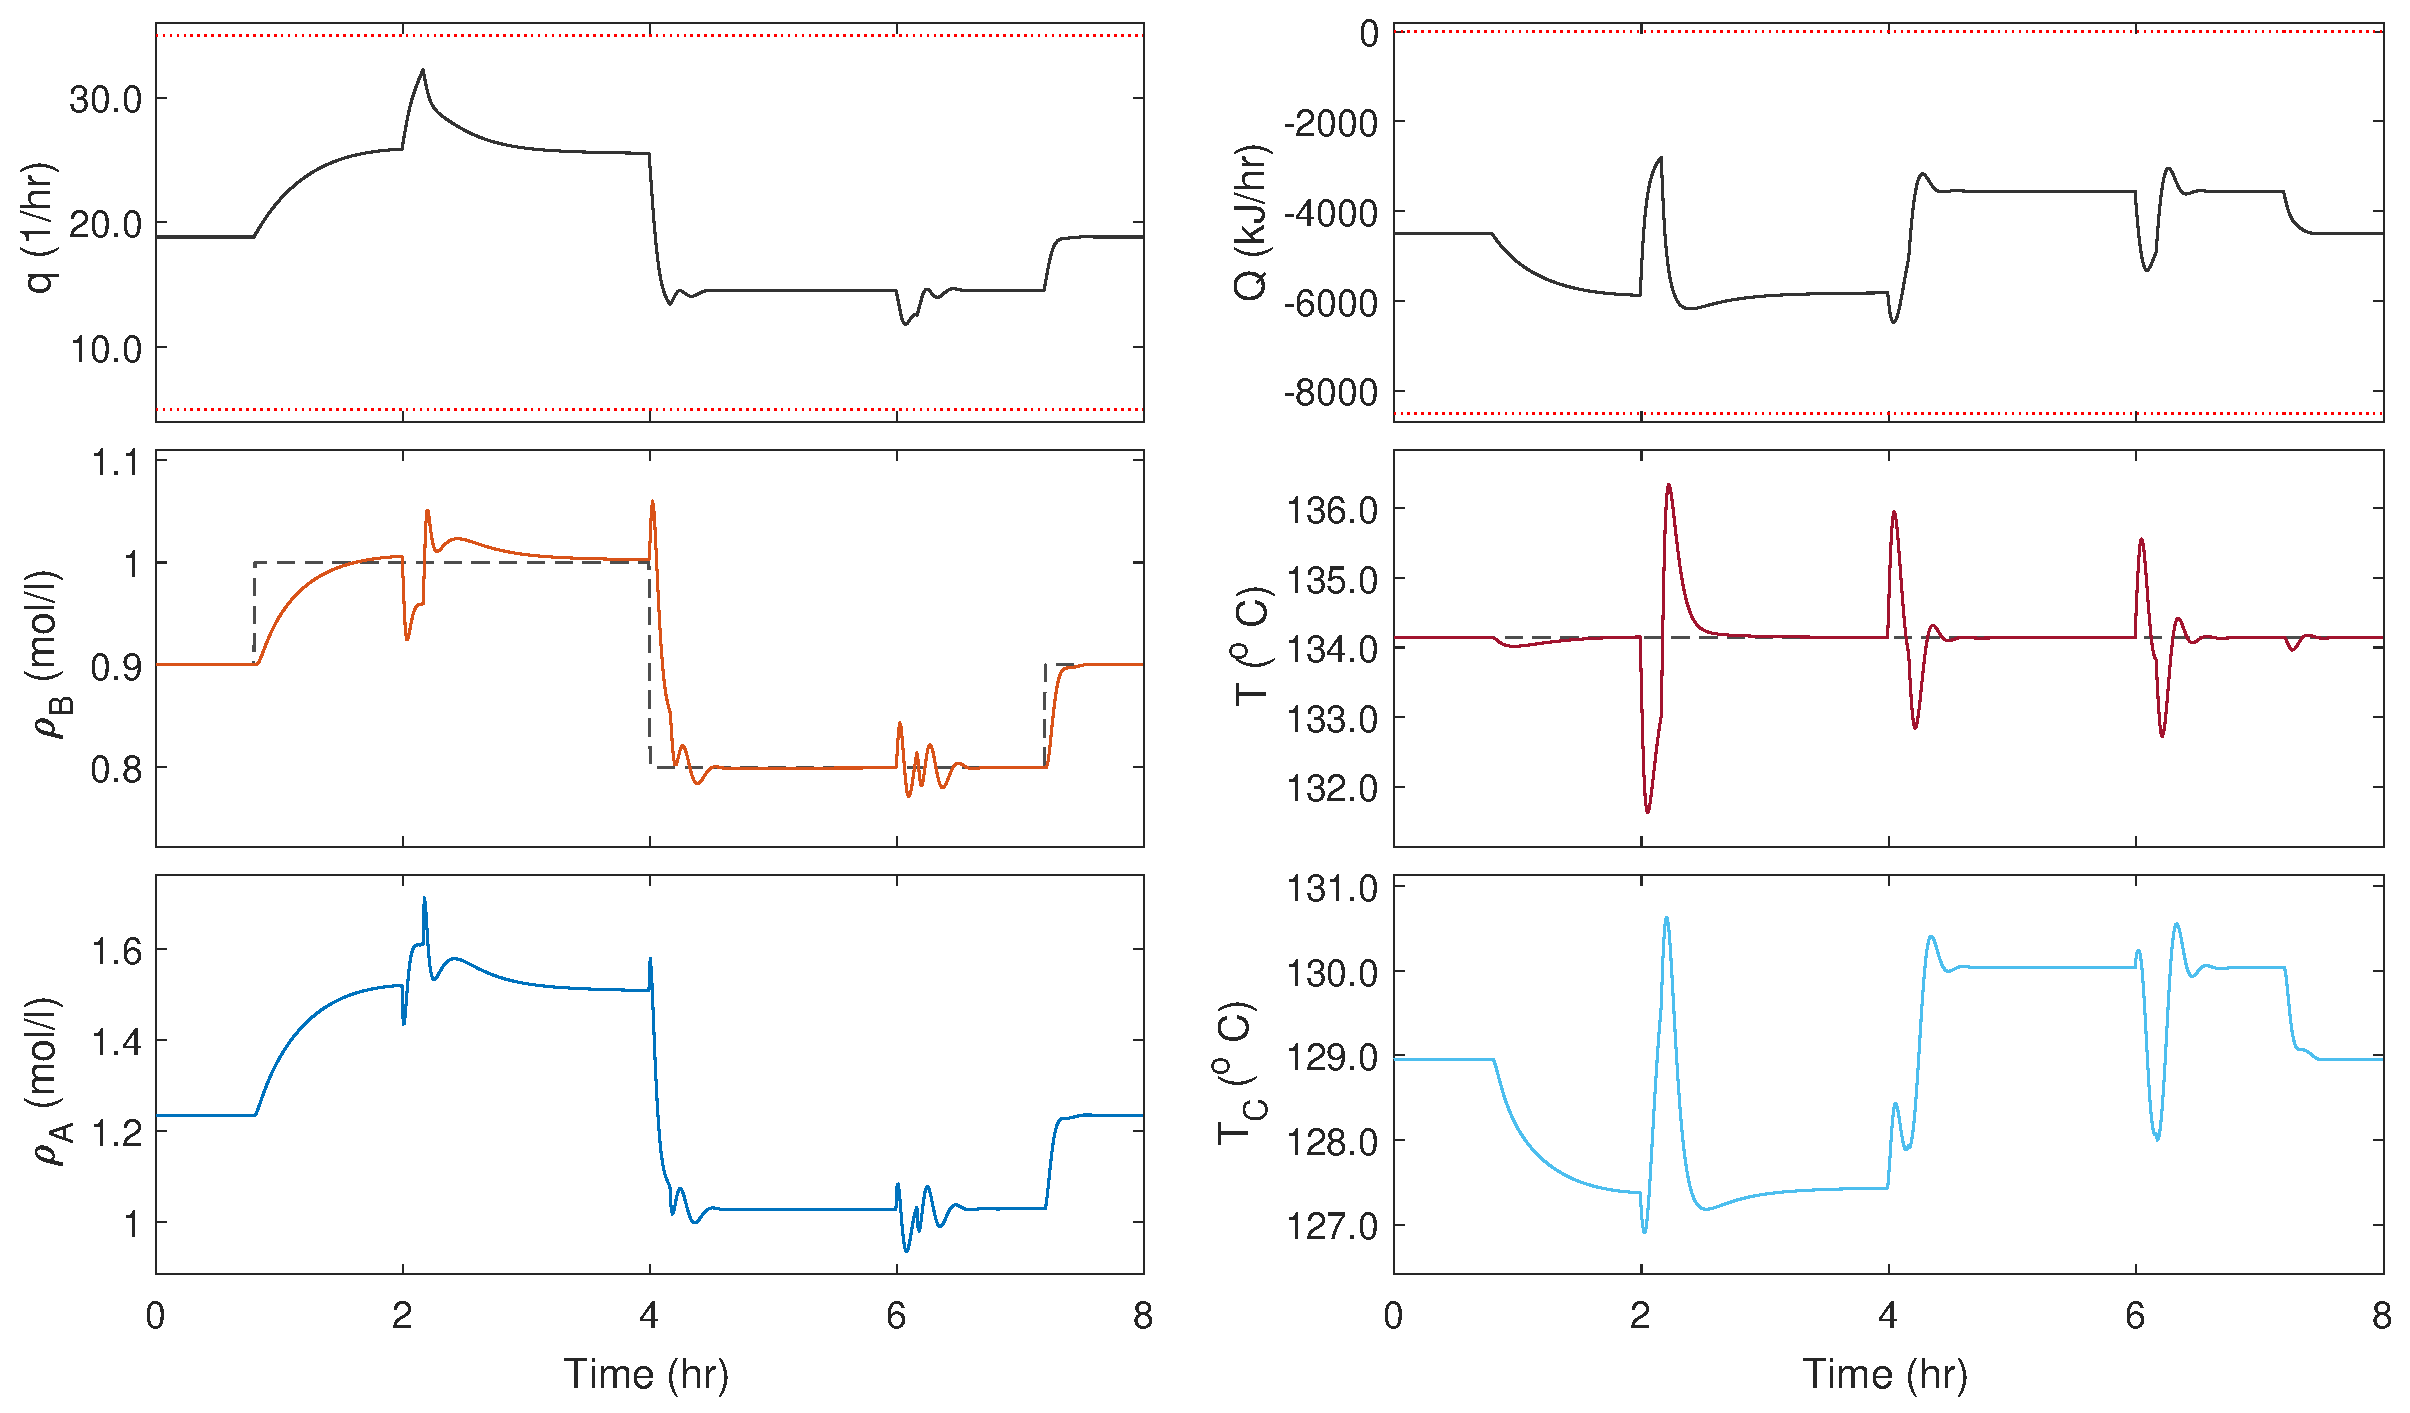
\includegraphics[width=\textwidth]{lqri02}
\end{figure}

\end{frame}

%-------------------------------------------------------
% SECTION - Optimal State Estimation
%-------------------------------------------------------
\section{Optimal State Estimation}
%-------------------------------------------------------
\subsection{Formulation}
%-------------------------------------------------------
\begin{frame}[t]{Optimal State Estimation}{Formulation}

\vskip0.25cm

\begin{varblock}[1\textwidth]{Closed-Loop Observer} 
    Given a system in State-Space with output signal $\bm{y}(t) : \mathbb{R} \rightarrow \mathbb{R}^p$ and an observer gain $\bm{L} \in \mathbb{R}^{n \times p}$, the estimated state-vector $\hat{\bm{x}}(t)$ is represented by the system:
    \begin{equation}
        \dot{\hat{\bm{x}}}(t) = \bm{A} \hat{\bm{x}}(t) + \bm{B} \bm{u}(t) + \bm{L} \left( \bm{y}(t) - \bm{C} \hat{\bm{x}}(t) \right)
    ,\end{equation}
    
    \noindent or, equivalently:
    \begin{equation}
        \dot{\hat{\bm{x}}}(t) = \left( \bm{A} - \bm{L} \bm{C} \right) \hat{\bm{x}}(t) + \bm{B} \bm{u}(t) + \bm{L} \bm{y}(t)
    .\end{equation} \vskip0.2cm
\end{varblock}

\begin{itemize}
	\item The observer system works as a parallel system that is simulated alongside the actual system; \vskip0.2cm
	
	\item Alternatively, it is possible to create a variable $\bm{e}(t) = \bm{x}(t) - \hat{\bm{x}}(t)$ such that:
	\begin{align}
	\begin{split}
	    \dot{\bm{e}} &= \bm{x} - \hat{\bm{x}} \\ 
	        &= \left( \bm{A} - \bm{L} \bm{C} \right) \left( \bm{x} - \hat{\bm{x}} \right) \\
	        &= \left( \bm{A} - \bm{L} \bm{C} \right) \bm{e},
	\end{split}
	\end{align}
	
	\noindent implying that the observer tracks the actual state-vector if $\bm{e}(t) = \bm{0}$ as $t \to \infty$.
\end{itemize}

\end{frame}

%-------------------------------------------------------
\begin{frame}[t]{Optimal State Estimation}{Formulation}

\vskip0.25cm

\begin{varblock}[1\textwidth]{Pole-Placement Property of Observers} 
    If a system in State-Space representation is observable, then by a closed-loop observer with gain matrix $\bm{L} \in \mathbb{R}^{n \times p}$ the eigenvalues of $\bm{A}_{obs} = \bm{A} - \bm{L} \bm{C}$ can arbitrarily be assigned anywhere in the complex plane, as long as that complex conjugate eigenvalues are assigned in pairs.
\end{varblock}

\begin{itemize}
	\item a
\end{itemize}

\end{frame}

%-------------------------------------------------------
\begin{frame}[t]{Optimal State Estimation}{Formulation}

\vskip0.25cm

\begin{varblock}[1\textwidth]{The Separation Principle} 
    Given a system in State-Space with a Luenberger observer of gain $\bm{L}$ and state-feedback controller of gain $\bm{K}$, the closed-loop eigenvalues contributions of $(\bm{A} - \bm{B}\bm{K})$ are independent from those of $(\bm{A} - \bm{L}\bm{C})$.
\end{varblock}

\begin{itemize}
	\item a
\end{itemize}

\end{frame}

%-------------------------------------------------------
\subsection{Kalman Filter and LQG Controllers}
%-------------------------------------------------------
\begin{frame}[t]{Optimal State Estimation}{Kalman Filter and Linear Quadratic Gaussian (LQG)}

\vskip0.25cm

\begin{varblock}[1\linewidth]{Kalman-Bucy Optimal Filter}
	Consider a continuous-time State-Space linear system subject to additive process noise variable $\bm{w}_k \sim \mathcal{N}(\bm{0}, \bm{Q}_{kf})$ and measurement noise variable $\bm{v}_k \sim \mathcal{N}(\bm{0}, \bm{R}_{kf})$, where the covariances $\bm{Q}_{kf} \in \mathbb{R}^{n \times n}$  and $\bm{R}_{kf} \in \mathbb{R}^{p \times p}$ represents the \emph{power spectral density} of the noises. In this case, for an estimated state $\bar{\bm{x}}(t)$ at time $t$, the error covariance:
    \begin{equation}
        \bm{J}(\bm{x}, \bar{\bm{x}}, t) = \mathbb{E}\left\{ [\bm{x}(t) - \bar{\bm{x}}(t)][\bm{x}(t) - \bar{\bm{x}}(t)]^T \right\}
    \end{equation}
    
    \noindent is minimized by $\bar{\bm{x}}(t)$ obtained through the system:
    \begin{equation}
        \dot{\bar{\bm{x}}}(t) = \bm{A} \bar{\bm{x}}(t) + \bm{B} \bm{u}(t) + \bm{K}_{e}(t) \left( \bm{y}(t) - \bm{C} \bar{\bm{x}}(t) \right)
    ,\end{equation}
    
    \noindent where $\bm{K}_e(t) = \bm{P}_e(t)\bm{C}\bm{R}^{-1}$, being $\bm{P}_e(t)$ the solution of the Riccati differential matrix equation:
    \begin{equation}
        \dot{\bm{P}_e}(t) = \bm{A} \bm{P}_e(t) + \bm{P}_e(t) \bm{A}^T - \bm{P}_e(t)\bm{C}^T\bm{R}_{kf}^{-1} \bm{C} \bm{P}_e(t) + \bm{Q}_{kf}
    ,\end{equation}
    
    \noindent with initial condition $\bm{P}_e(t_0) = \mathbb{E} \left\{ [\bm{x}(t_0) - \bar{\bm{x}}(t_0)][\bm{x}(t_0) - \bar{\bm{x}}(t_0)]^T \right\}$ for $t_0 > -\infty$.
\end{varblock}

\end{frame}

%-------------------------------------------------------
\begin{frame}[t]{Optimal State Estimation}{Kalman Filter and Linear Quadratic Gaussian (LQG)}

\vskip0.25cm

\begin{varblock}[1\linewidth]{Linear Quadratic Gaussian (LQG) Controller}
	Consider a stochastic system in State-Space representation:
	\begin{align}
    \begin{cases}
        \hfill \dot{\bm{x}}(t) &= \bm{A} \bm{x}(t) + \bm{B} \bm{u}(t) + \bm{w}(t) \\
        \hfill \bm{y}(t) &= \bm{C} \bm{x}(t) + \bm{v}(t)
    \end{cases}
    ,\end{align}
    
     \noindent whose estimated state-vector $\hat{\bm{x}}(t)$ is determined by a Kalman-Bucy filter and whose optimal input signal $\bm{u}(t)$ is calculated through a finite-horizon LQR. The Linear Quadratic Gaussian (LQG) control for the horizon $t \in [t_0, T]$, with $-\infty < t_0 \leq T < \infty$, is defined as:
    \begin{align} 
        \dot{\hat{\bm{x}}}(t) = \left[\bm{A} - \bm{K}_e(t) \bm{C} - \bm{B} \bm{K}(t) \right] \hat{\bm{x}}(t) + \bm{K}_e(t) \bm{y}(t) 
    ,\end{align}
    
    \noindent where $\bm{K}(t) = \bm{R}^{-1}\bm{B}^T \bm{P}(t)$ and $\bm{K}_e(t) = \bm{P}_e(t) \bm{C} \bm{R}^{-1}$ are, respectively, the LQR and Kalman-Bucy gains for matrices $\bm{P}(t)$ and $\bm{P}_e(t)$ that solve the Riccati differential equations:
    \begin{align}
    \begin{cases}
        -\dot{\bm{P}}(t) = \bm{A}^T \bm{P}(t) + \bm{P}(t) \bm{A} - \bm{P}(t) \bm{B} \bm{R}^{-1} \bm{B}^T \bm{P}(t) + \bm{Q} \\
        \phantom{-} \dot{\bm{P}_e}(t) = \bm{A} \bm{P}_e(t) + \bm{P}_e(t) \bm{A}^T - \bm{P}_e(t)\bm{C}^T\bm{R}_{kf}^{-1} \bm{C} \bm{P}_e(t) + \bm{Q}_{kf}
    \end{cases}
    \end{align}
    
    \noindent for boundary conditions $\bm{P}(T) = \bm{Q}_f$ and $\bm{P}_e(t_0) = \mathbb{E} \left\{ [\bm{x}(t_0) - \bar{\bm{x}}(t_0)][\bm{x}(t_0) - \bar{\bm{x}}(t_0)]^T \right\}$, respectively.
\end{varblock}

\end{frame}

%-------------------------------------------------------
\begin{frame}[c]{Optimal State Estimation}{Kalman Filter and Linear Quadratic Gaussian (LQG)}

\vskip0.25cm

\begin{figure}[ht]
    \centering
    \resizebox{0.9\textwidth}{!}{
    \begin{tikzpicture}[auto, node distance=1.75cm,>=latex']
        % We start by placing the blocks
        \node [input, name=input] {};
        \node [sum, right of=input, node distance=3em] (intFbckSum) {};
        \node [block, right of=intFbckSum, node distance=4em] (integralAction) {$\int$};
        \node [block, right of=integralAction, node distance=6em] (intActGain) {$\bm{K}_a$};
        \node [sum, right of=intActGain, node distance=4.5em] (fbckSum) {};

        \node [block, fill=glgBlue!20, minimum height=4em, right of=fbckSum, node distance=14em] (openloopSystem) {Open-Loop System};    
        \node [output, right of=outputMatrix, node distance=10em] (output) {};
        
        \node [block, below of=openloopSystem, node distance=14em] (integralLU) {$\int$};     
        \node [sum, left of=integralLU, node distance=4em] (stateSumLU) {};             
        \node [block, left of=stateSumLU, node distance=4em] (inputMatrixLU) {$\bm{B}$};
        \node [block, right of=integralLU, node distance=8em] (outputMatrixLU) {$\bm{C}$};
        \node [block, below of=integralLU] (stateMatrixLU) {$\bm{A}$};
        \node [block, above of=integralLU] (kalmanGain) {$\bm{K}_e$};       
        
        \draw [->] (openloopSystem) -- node[name=bk3,pos=0.5]{} node[name=bk5,pos=0.75]{} node[pos=0.9]{$\bm{y}$} (output);
        \node [sum, anchor=base] (fbckOutput) at (bk3.base |- kalmanGain) {};
        
        \node [block, below of=stateSumLU, node distance=12em, label={below:LQR Controller}] (fbckGain) {$\bm{K}$};     
        
        
        \begin{scope}[on background layer]
            \node [fit=(integralAction) (intActGain), fill= glgGreen!10, rounded corners, inner sep=.4cm, label={[xshift=4.3em, glgGreen!90]above left:Integral Action}] {};
        \end{scope} 
        
        \begin{scope}[on background layer]
            \node [fit=(inputMatrixLU) (kalmanGain) (stateMatrixLU) (fbckOutput), fill= glgRed!10, rounded corners, inner sep=.4cm, label={[xshift=5.75em, glgRed!90]above left:Kalman-Bucy Filter}] {};
        \end{scope} 
        
        % Once the nodes are placed, connecting them is easy.       
        \draw [draw,->] (input) -- node[pos=0.1] {$\bm{r}$} node[pos=0.8] {$+$}  (intFbckSum);
        \draw [->] (intFbckSum) -- (integralAction);
        \draw [->] (integralAction) -- node[pos=0.5]{$\bm{x}_a$} (intActGain);
        \draw [->] (intActGain) -- node[pos=0.8]{$-$} (fbckSum);        
        \draw [->] (fbckSum) -- node[pos=0.2]{$\bm{u}$} node[name=bku1, pos=0.2]{} (openloopSystem);
        

        \draw [->] (fbckGain) -| node[pos=0.98]{$-$} (fbckSum);
        \draw [->] (bk5) |- ++(0, -30em) -| node[pos=0.98]{$-$} (intFbckSum);
        
        
        \draw [->] (bku1) |- (inputMatrixLU);
        \draw [->] (inputMatrixLU) -- node[pos=0.8]{$+$} (stateSumLU);
        \draw [->] (stateSumLU) -- node[pos=0.5]{$\dot{\hat{\bm{x}}}$} (integralLU);
        \draw [->] (integralLU) -- node[name=bk4,pos=0.5]{} node[pos=0.5]{$\hat{\bm{x}}$} (outputMatrixLU);
        \draw [->] (outputMatrixLU) -| node[pos=0.95]{$-$} (fbckOutput);
        \draw [->] (bk4) |- (stateMatrixLU);
        \draw [->] (fbckOutput) -- (kalmanGain);
        \draw [->] (stateMatrixLU) -| node[pos=0.95]{$+$} (stateSumLU);
        \draw [->] (kalmanGain) -| node[pos=0.95]{$+$} (stateSumLU);
        \draw [->] (bk3) -- node[pos=0.95]{$+$} (fbckOutput);
        
        \draw [->] (bk4) |- (fbckGain);
    \end{tikzpicture} 
    }
\end{figure}

\end{frame}

%-------------------------------------------------------
\subsection{Simulations}
%-------------------------------------------------------
\begin{frame}[c]{Optimal Control}{Simulations}

\vskip0.25cm

\begin{figure}[h]
	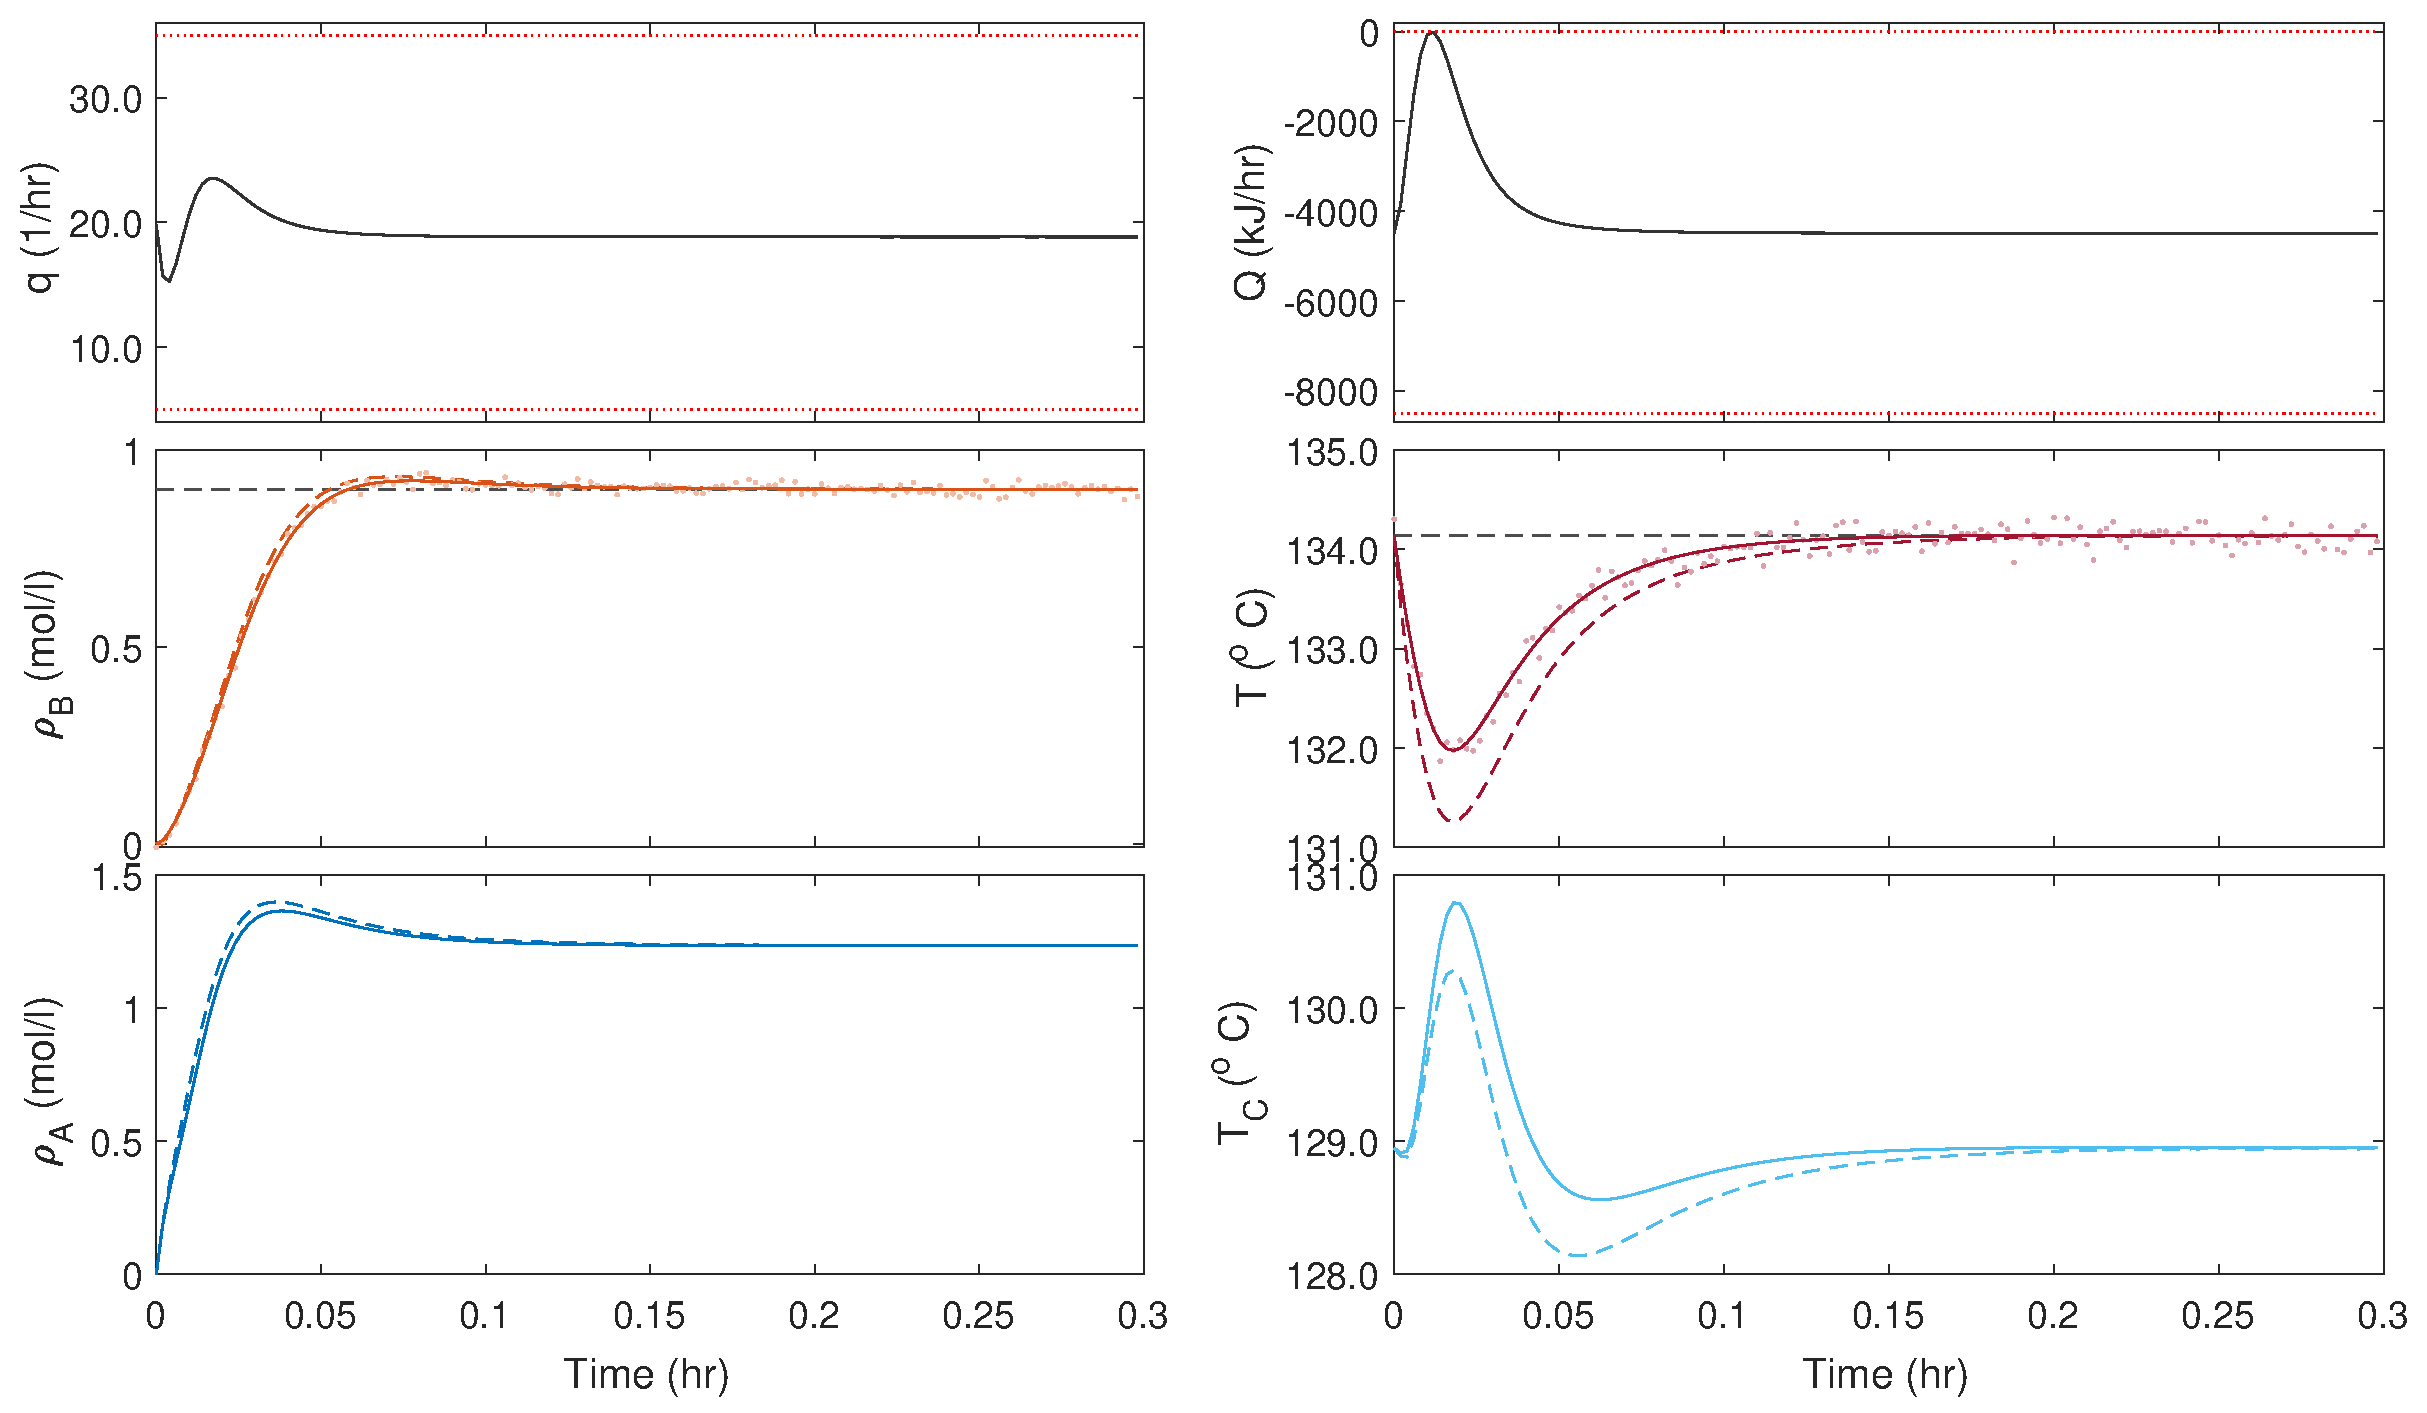
\includegraphics[width=\textwidth]{lqg01}
\end{figure}

\end{frame}

%-------------------------------------------------------
\begin{frame}[c]{Optimal Control}{Simulations}

\vskip0.25cm

\begin{figure}[h]
	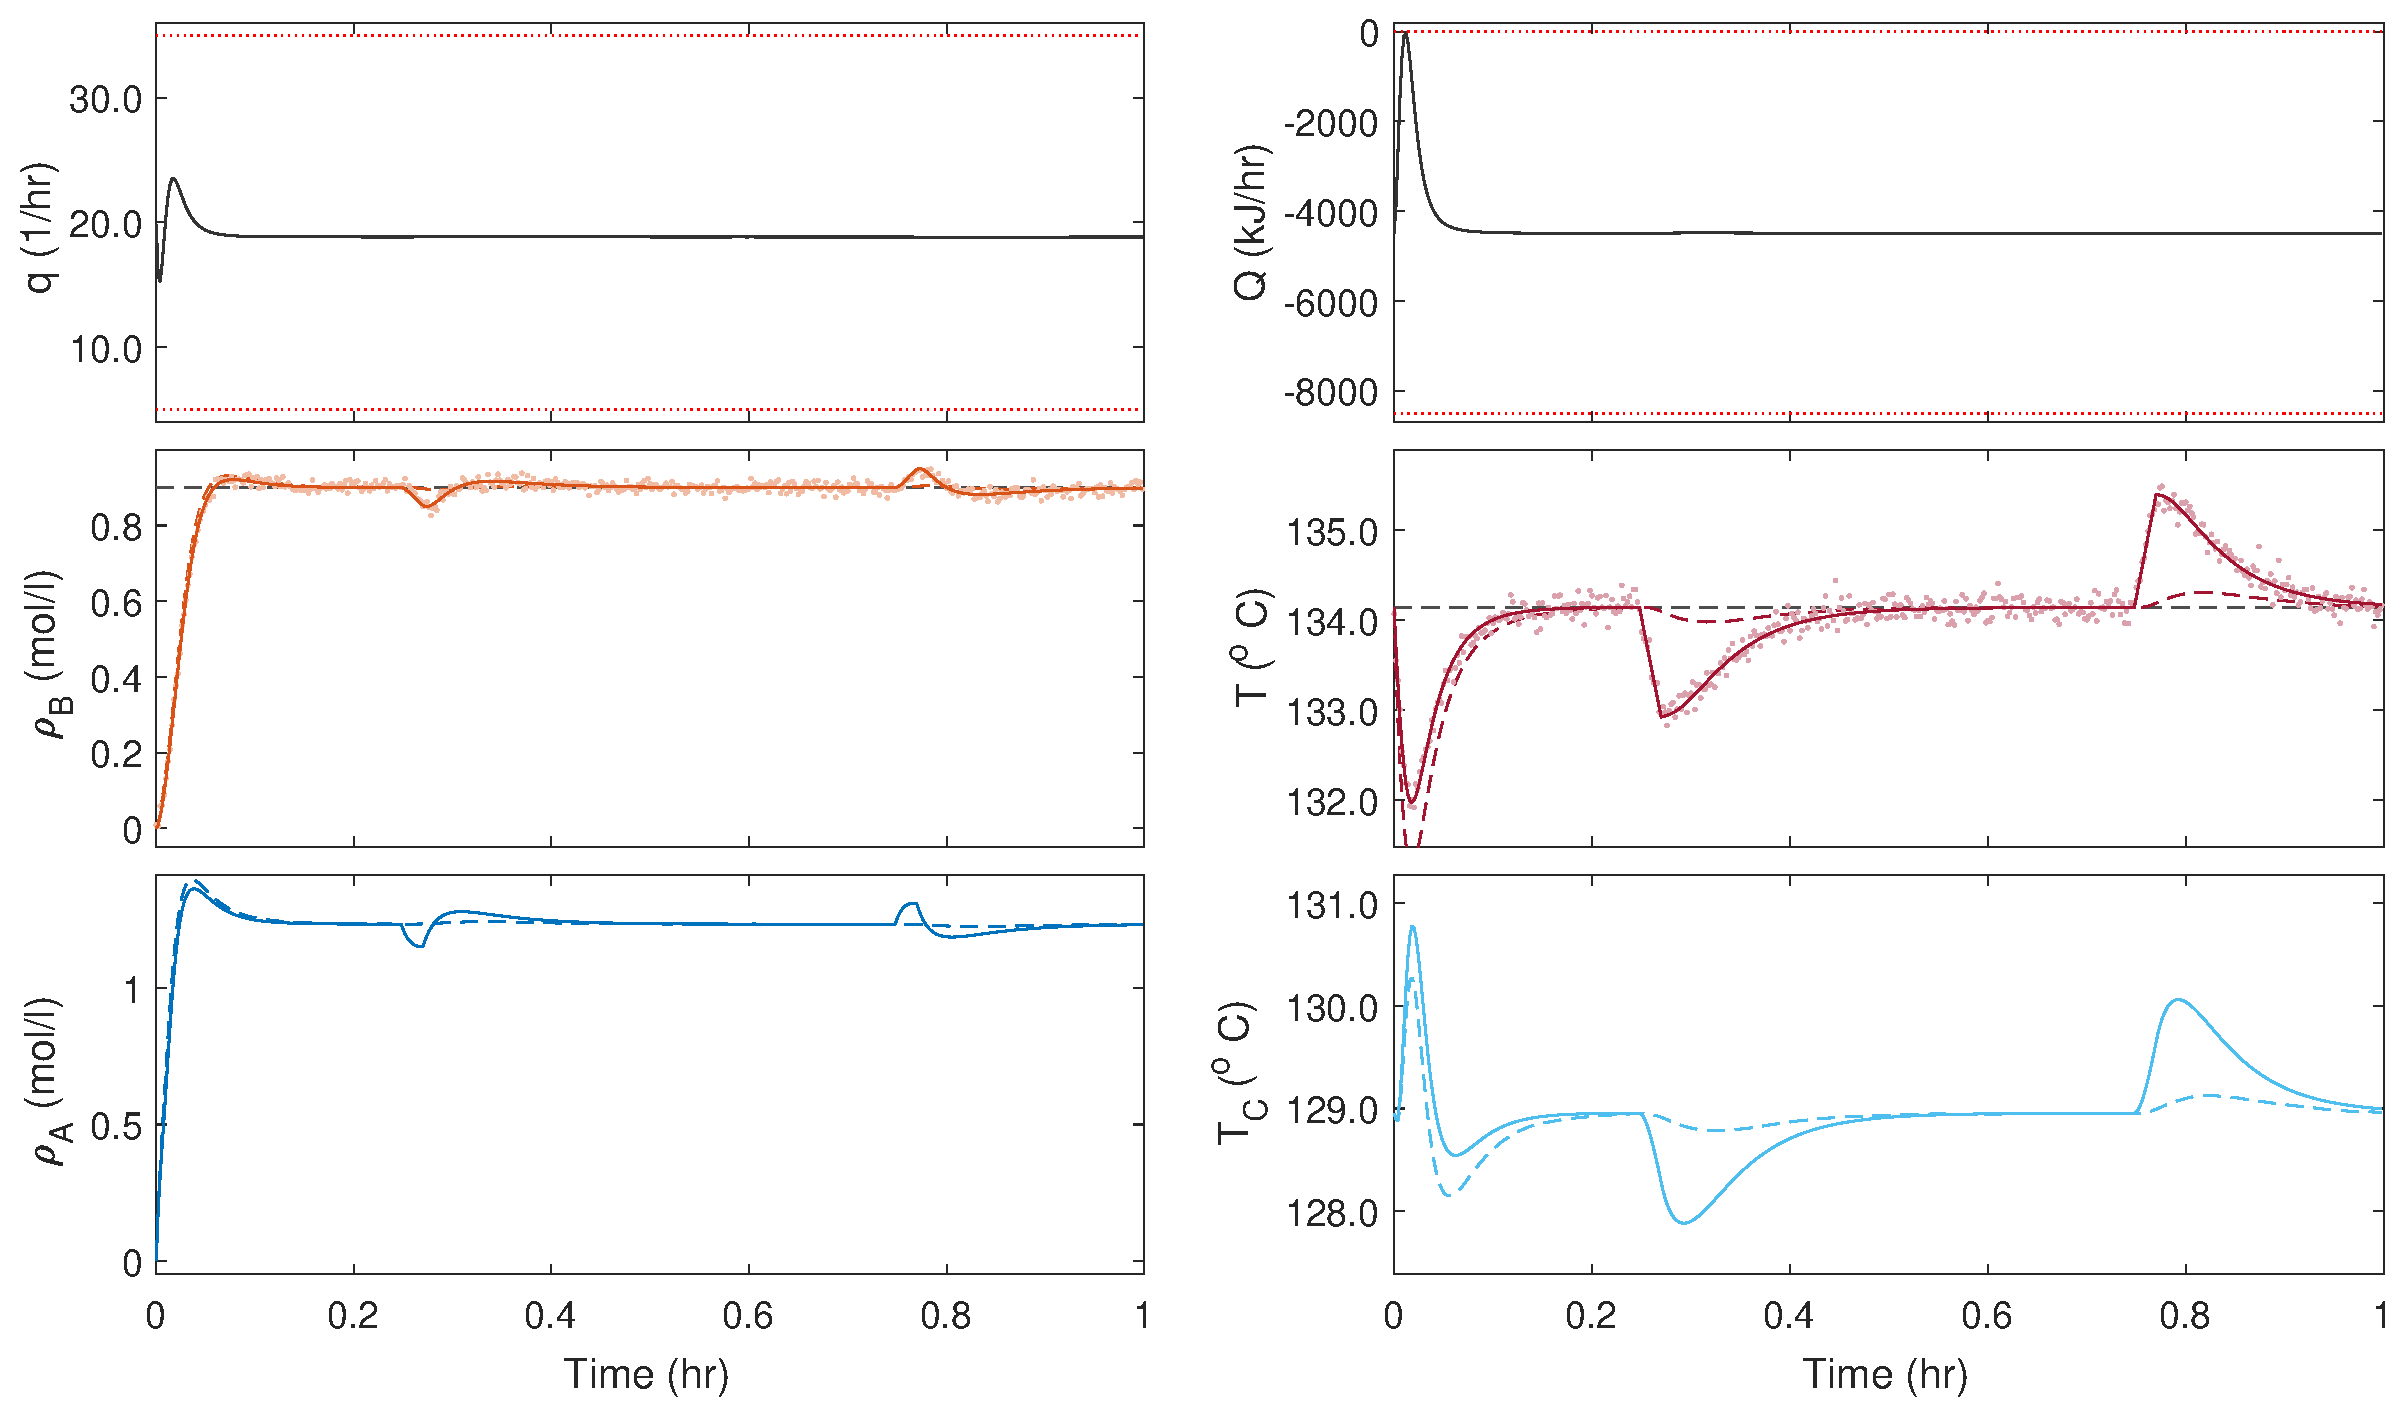
\includegraphics[width=\textwidth]{lqg02}
\end{figure}

\end{frame}

%-------------------------------------------------------
\begin{frame}[c]{Optimal Control}{Simulations}

\vskip0.25cm

\begin{figure}[h]
	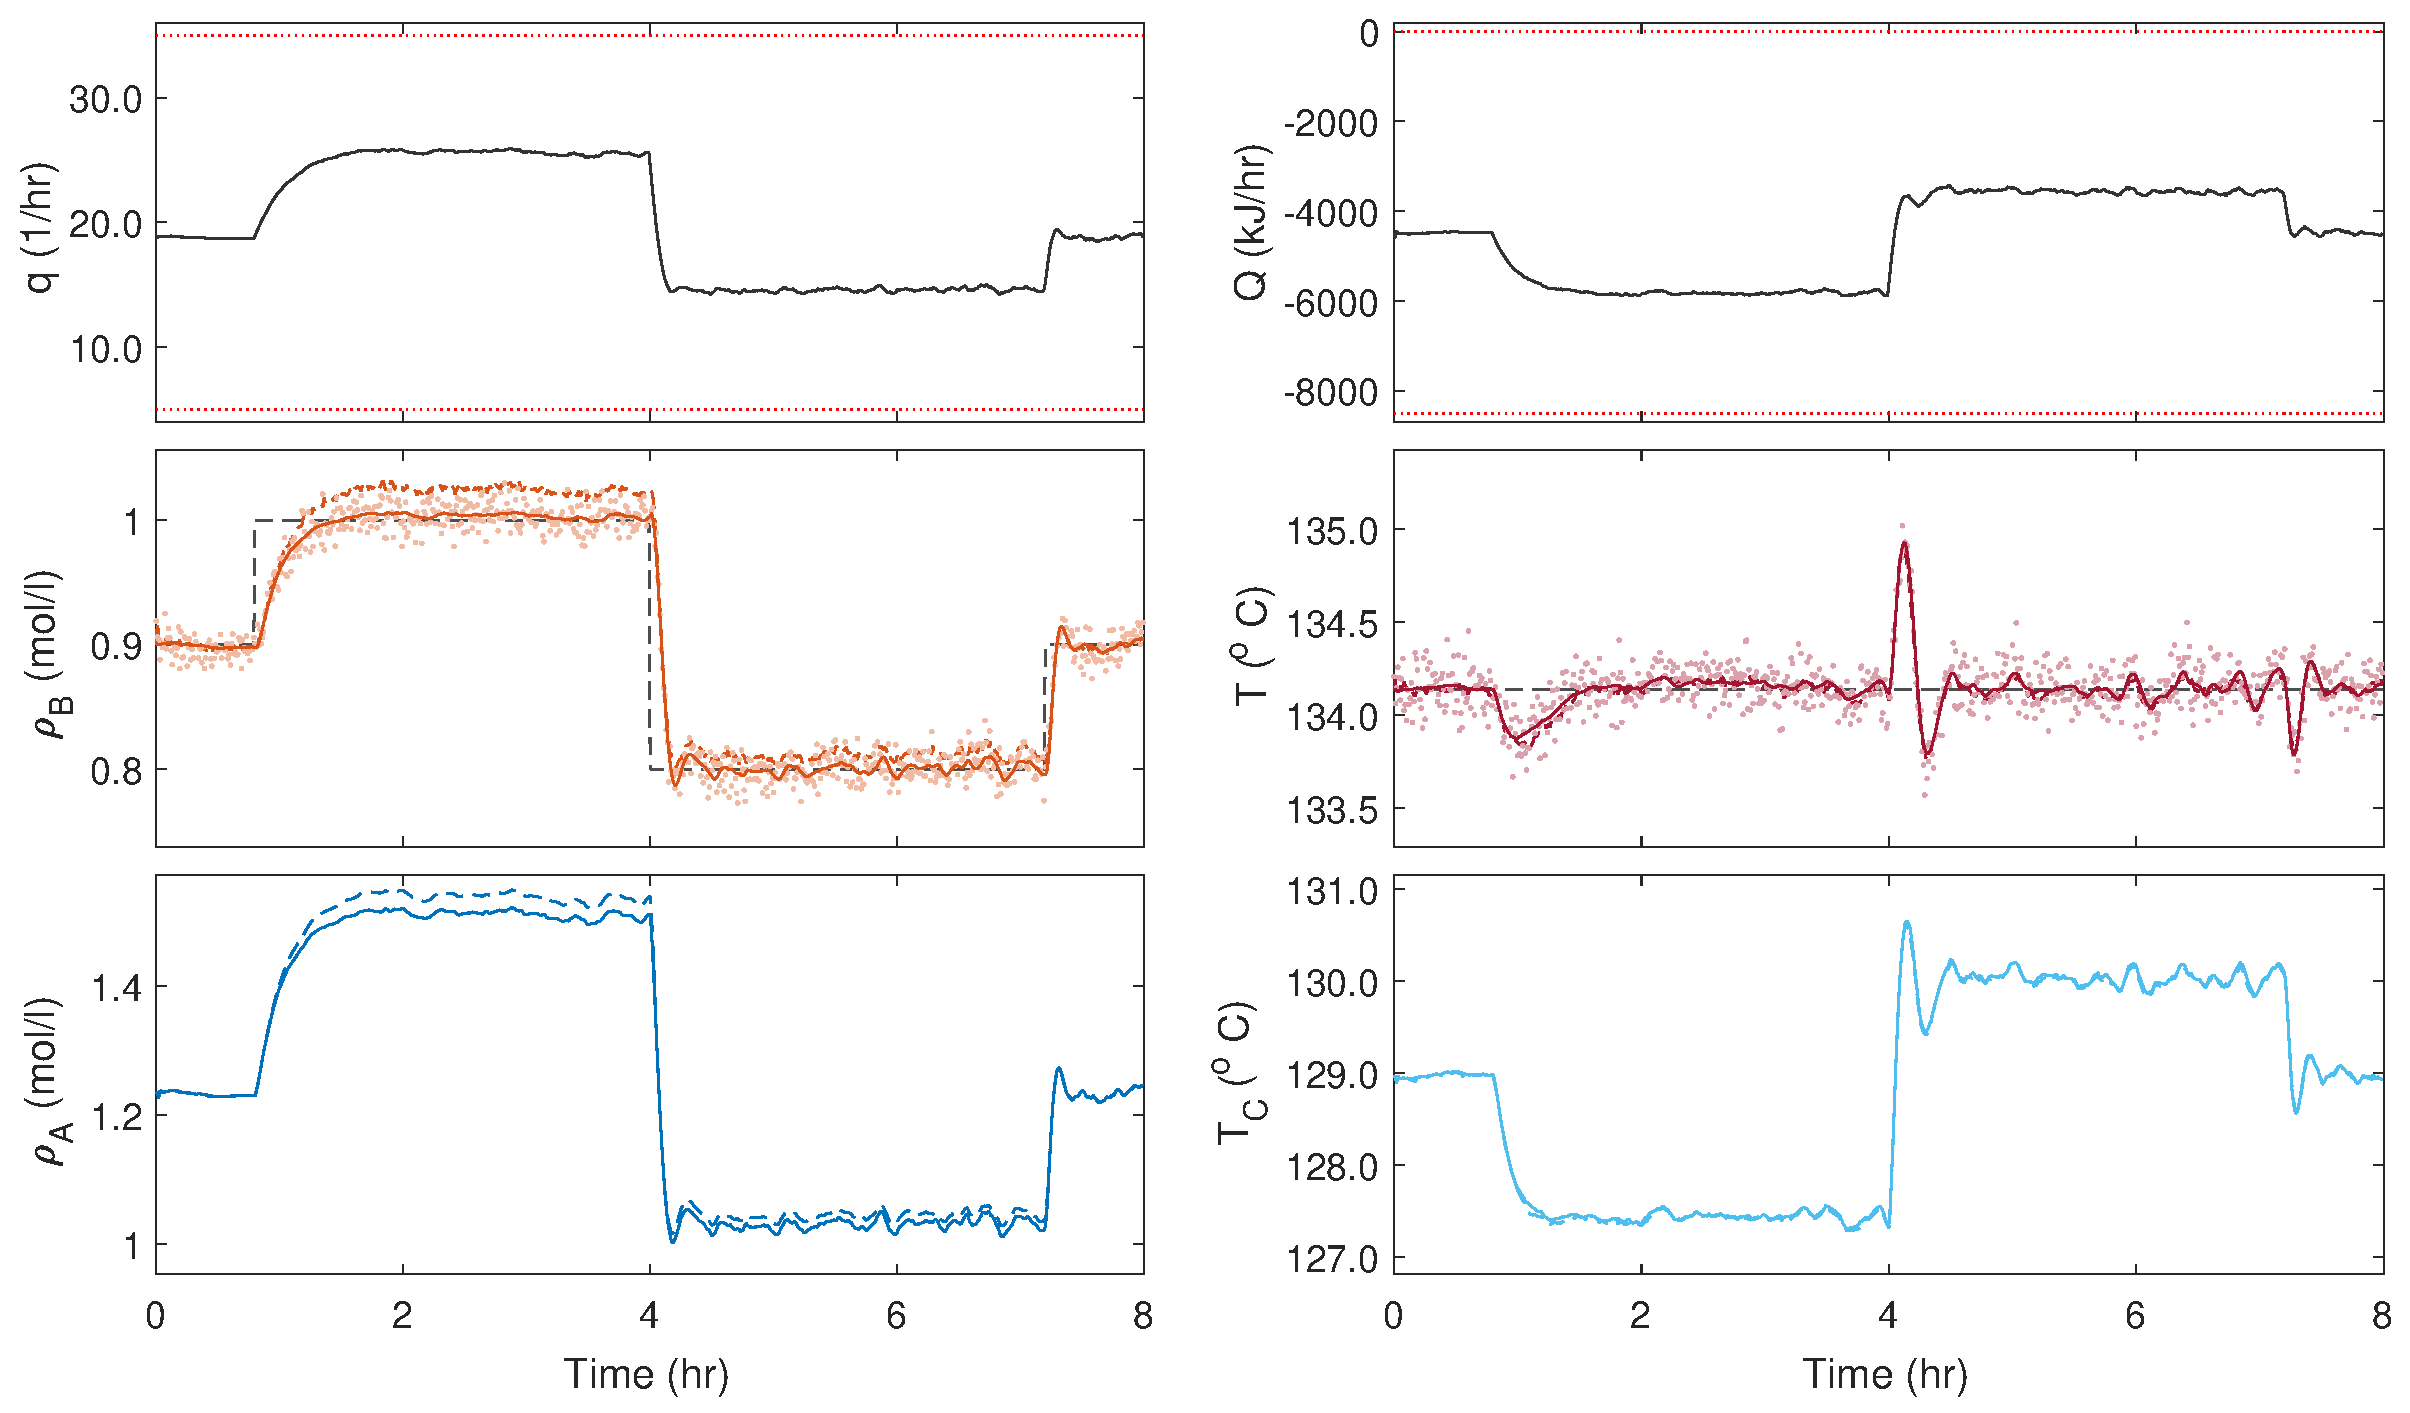
\includegraphics[width=\textwidth]{lqgi01}
\end{figure}

\end{frame}

%-------------------------------------------------------
\begin{frame}[c]{Optimal Control}{Simulations}

\vskip0.25cm

\begin{figure}[h]
	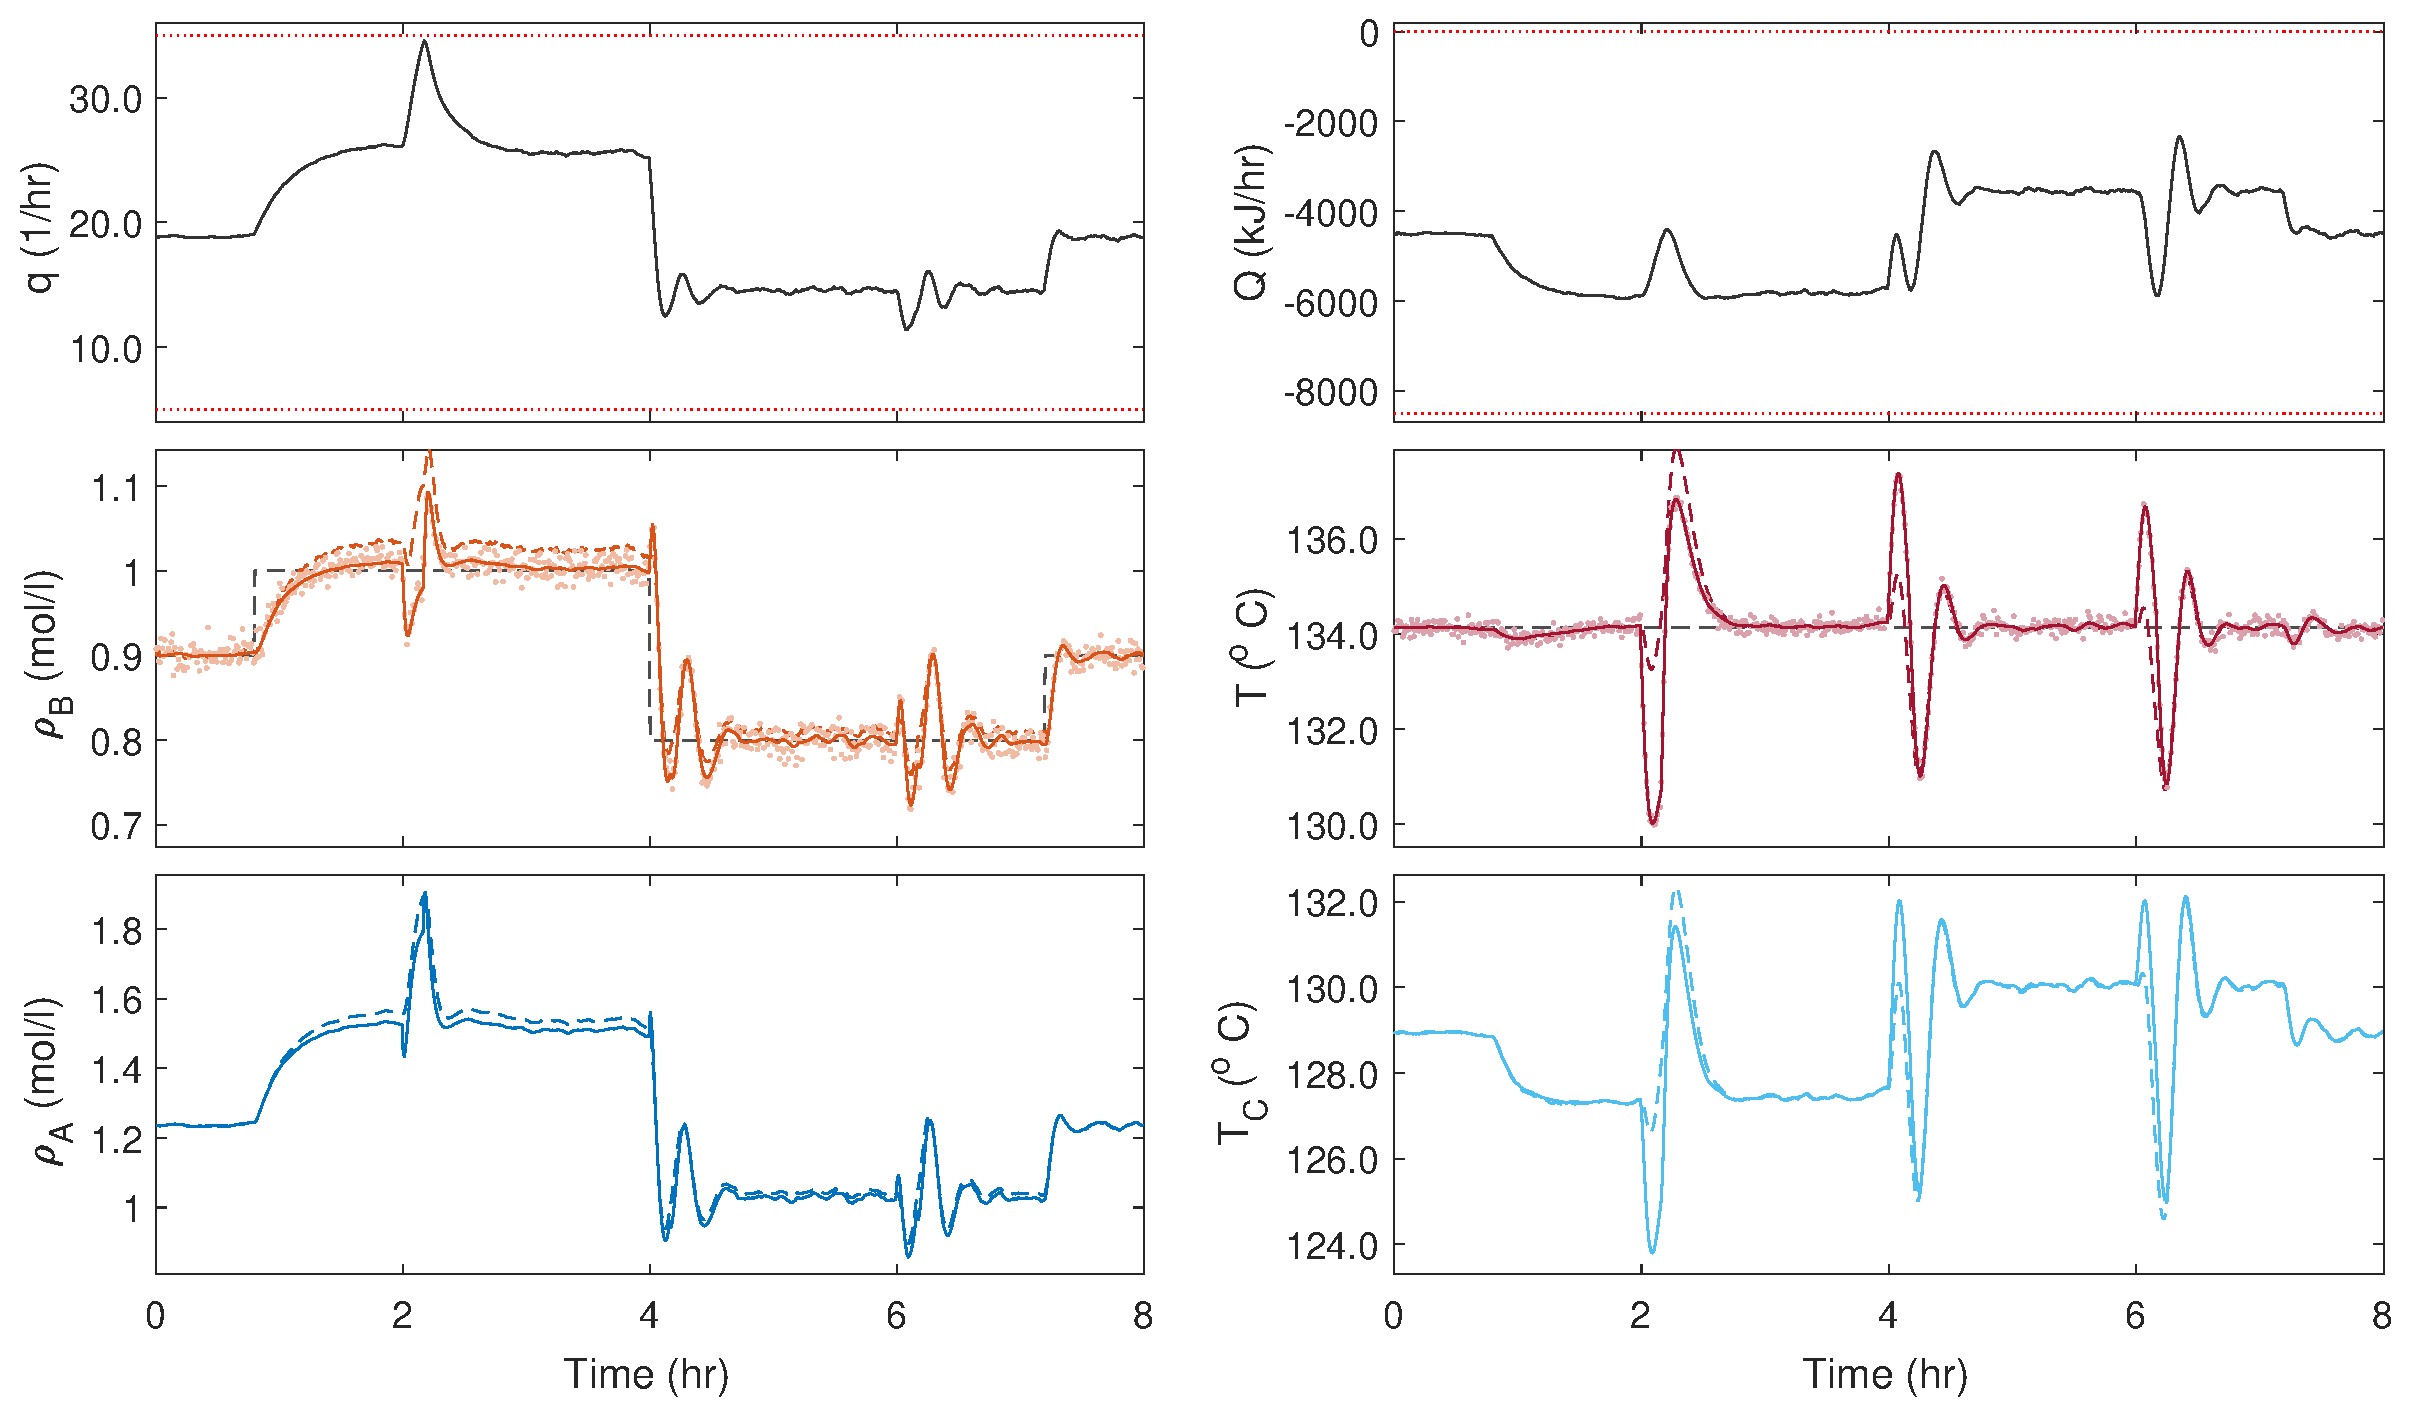
\includegraphics[width=\textwidth]{lqgi02}
\end{figure}

\end{frame}

%-------------------------------------------------------
% SECTION - Conclusion
%-------------------------------------------------------
\section{Conclusion}
%-------------------------------------------------------
\begin{frame}[t]{Conclusion}{}

\vskip0.25cm

\begin{itemize}
	\item Past;
	
	\item Present;
	
	\item Future;
\end{itemize}


\end{frame}

%-------------------------------------------------------
\begin{frame}[allowframebreaks] \small
        \frametitle{References}
        \bibliographystyle{apalike}
        \bibliography{citations.bib}
\end{frame}


%-------------------------------------------------------
%-- End Page
{\1
\begin{frame}[plain,noframenumbering]
	\center \Huge \textbf{Thank you!}    	  
	  
	Questions?
\end{frame}

%-------------------------------------------------------
\end{document}


%%---------------------Rascunho--------------------------
%\section{Titulo}
%\subsection{Subtitulo}
%%---------------------Rascunho--------------------------
%\begin{frame}{Titulo}{Subtitulo}
%
%\begin{block}{title}
%	Say somethings \alert{new} 
%\end{block}
%
%\begin{itemize}
%	\item TikZ\footnote{TikZ is a package for creating beautiful graphics. Have a look at these \chref{http://www.texample.net/tikz/examples/}{online examples} or the \chref{http://tug.ctan.org/tex-archive/graphics/pgf/base/doc/generic/pgf/pgfmanual.pdf}{pgf user manual}.}
%\end{itemize}
%
%\end{frame}
%%---------------------Rascunho--------------------------

%%%%%%%%%%%%%%%%%%%%%%%%%%%%%%%%%%%
%% Drafts:
%%%%%%%%%%%%%%%%%%%%%%%%%%%%%%%%%%%
%%%%% Figure:
% \begin{figure}[ht]
% 	\centering
% 	\includegraphics[trim={0cm 0cm 0cm 0cm},clip,scale=1]{nameFigure}
% 	\caption{caption of the figure.}
% 	\label{fig:nameFigure}
% \end{figure} \vskip0.25cm
%
%%%%% Equation:
% \begin{equation} \label{eq:nameEquation}
% \begin{split}
%	 X = 1 + 1
% \end{split}
% \end{equation} \vskip0.25cm
%
%%%% Table:
% \begin{table}[hp]
% 	\centering
% 	\begin{tabular}{l | c c }
% 	Principal & Coluna1 & Coluna2 \\
% 	\hline 
% 	ABC	& 1 & 2 \\
% 	DFG	& 3 & 4 \\
% 	HIJ	& 5 & 6 \\
% 	\end{tabular} 
% 	\caption{caption of the table.}
% 	\label{table:nameTable}	
% \end{table} \vskip0.25cm
